\chapter{Frontend Implementation}

\section{Architecture Overview}
    There are many reasons why we chose React in our project. First of all, everything in React is component which it consists of state (mutable) and props (immutable). It means that it will make your code more predictable and easier to debug. Another reason is that it uses virtual Document Object Model (virtual DOM) instead of using pure DOM. The virtual DOM help to re-render in an efficient way of the DOM. In addition, React will create virtual DOM in memory when the program work, React will renders only the sub-component that only change. 
    


\section{Implementation}
    
    \subsection{Logging into the System}
    
    User can log-in to the application by entering user name ans password, that provided by the developer team, as shown in the figure \ref{log-in}. After entering all user name and password, user have to click log-in button in order to enter to the application. Then the system will send user's credential to validate with server by using POST method to post /api/v1/auth/login with the data to server. If user succeed log-in, at a glance report page will be rendered as shown in figure \ref{at-a-glance-report}. Server will send the data of that user and cookie to the front-end part.
    
    
    \FloatBarrier
    	\begin{figure}[h!]
            \centering
                % can use width=\linewidth
        		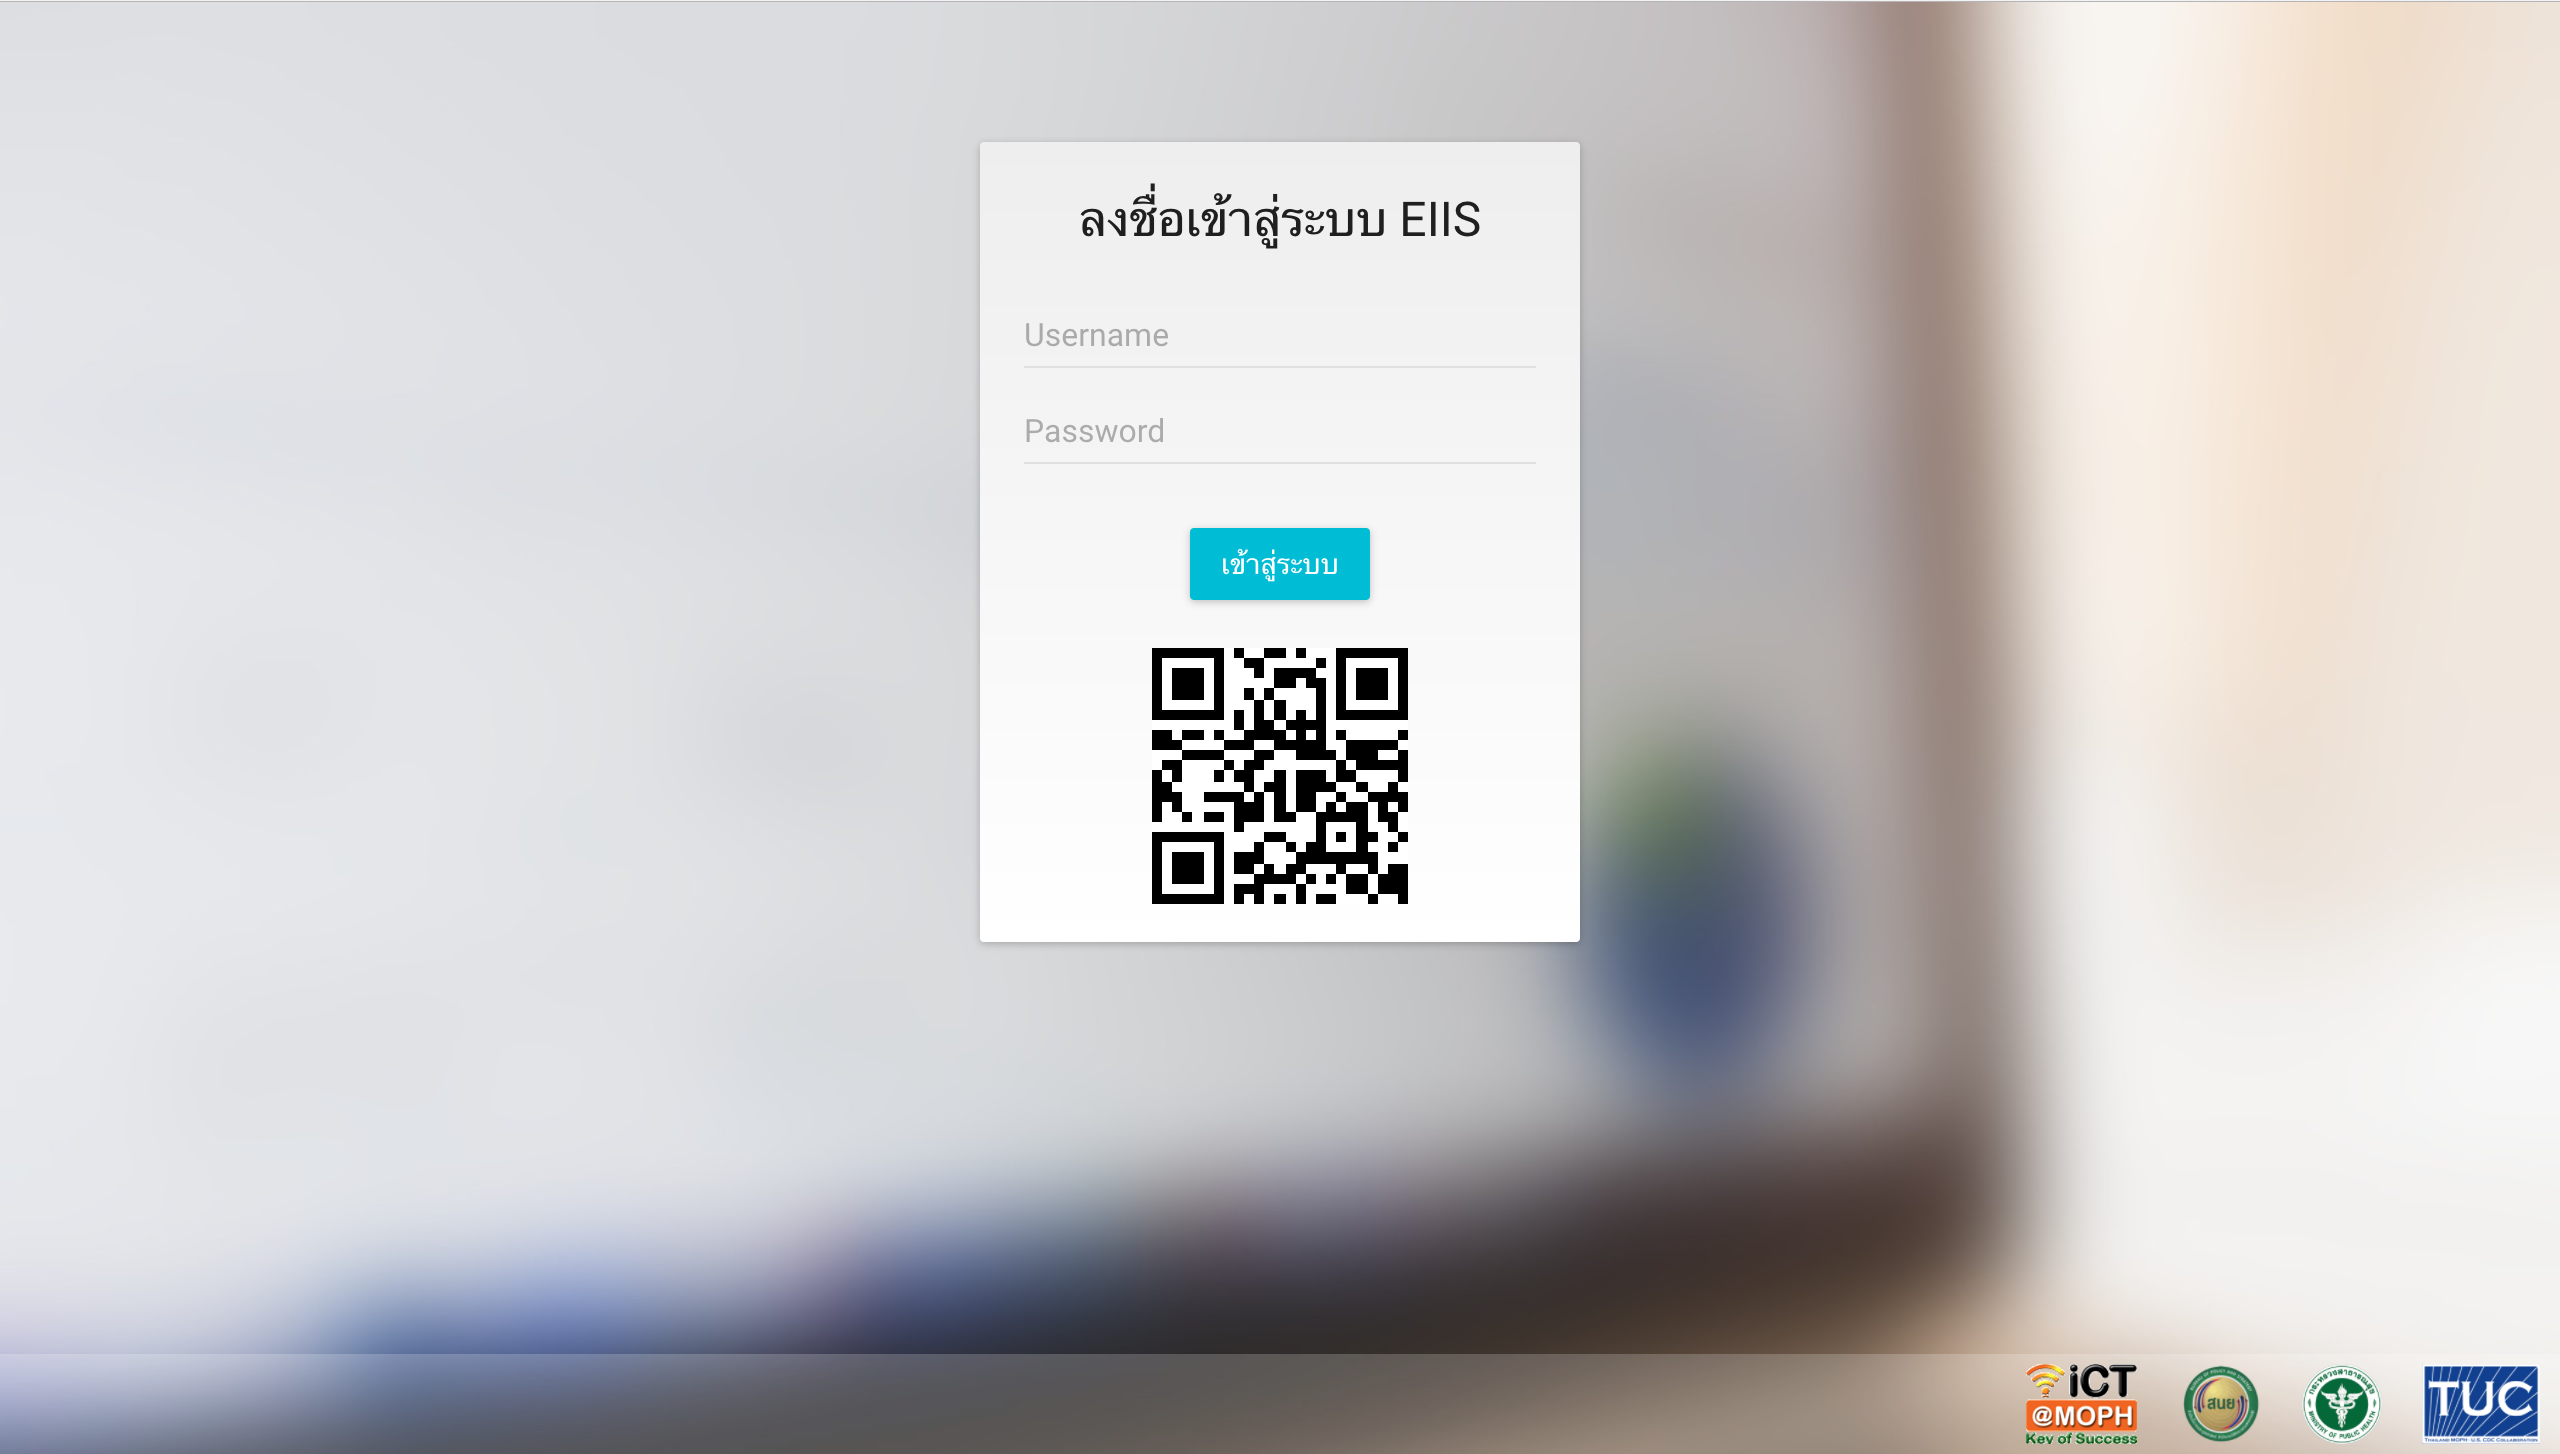
\includegraphics[width=12cm]{images/chapter-05/log-in.png}
        		\caption{Log-In Page}
        		\label{log-in}
        \end{figure}
	\FloatBarrier
	
	
	\subsection{Tab Bar Menu}
	
	This is all the menus that user can click to go to those pages. There are several pages in this application such as, home page, upload page, check upload status page, at a glance report page, demographics page, and so on. The tab bar menu shown in figure \ref{tab-bar-menu}
	
	\FloatBarrier
    	\begin{figure}[h!]
            \centering
                % can use width=\linewidth
        		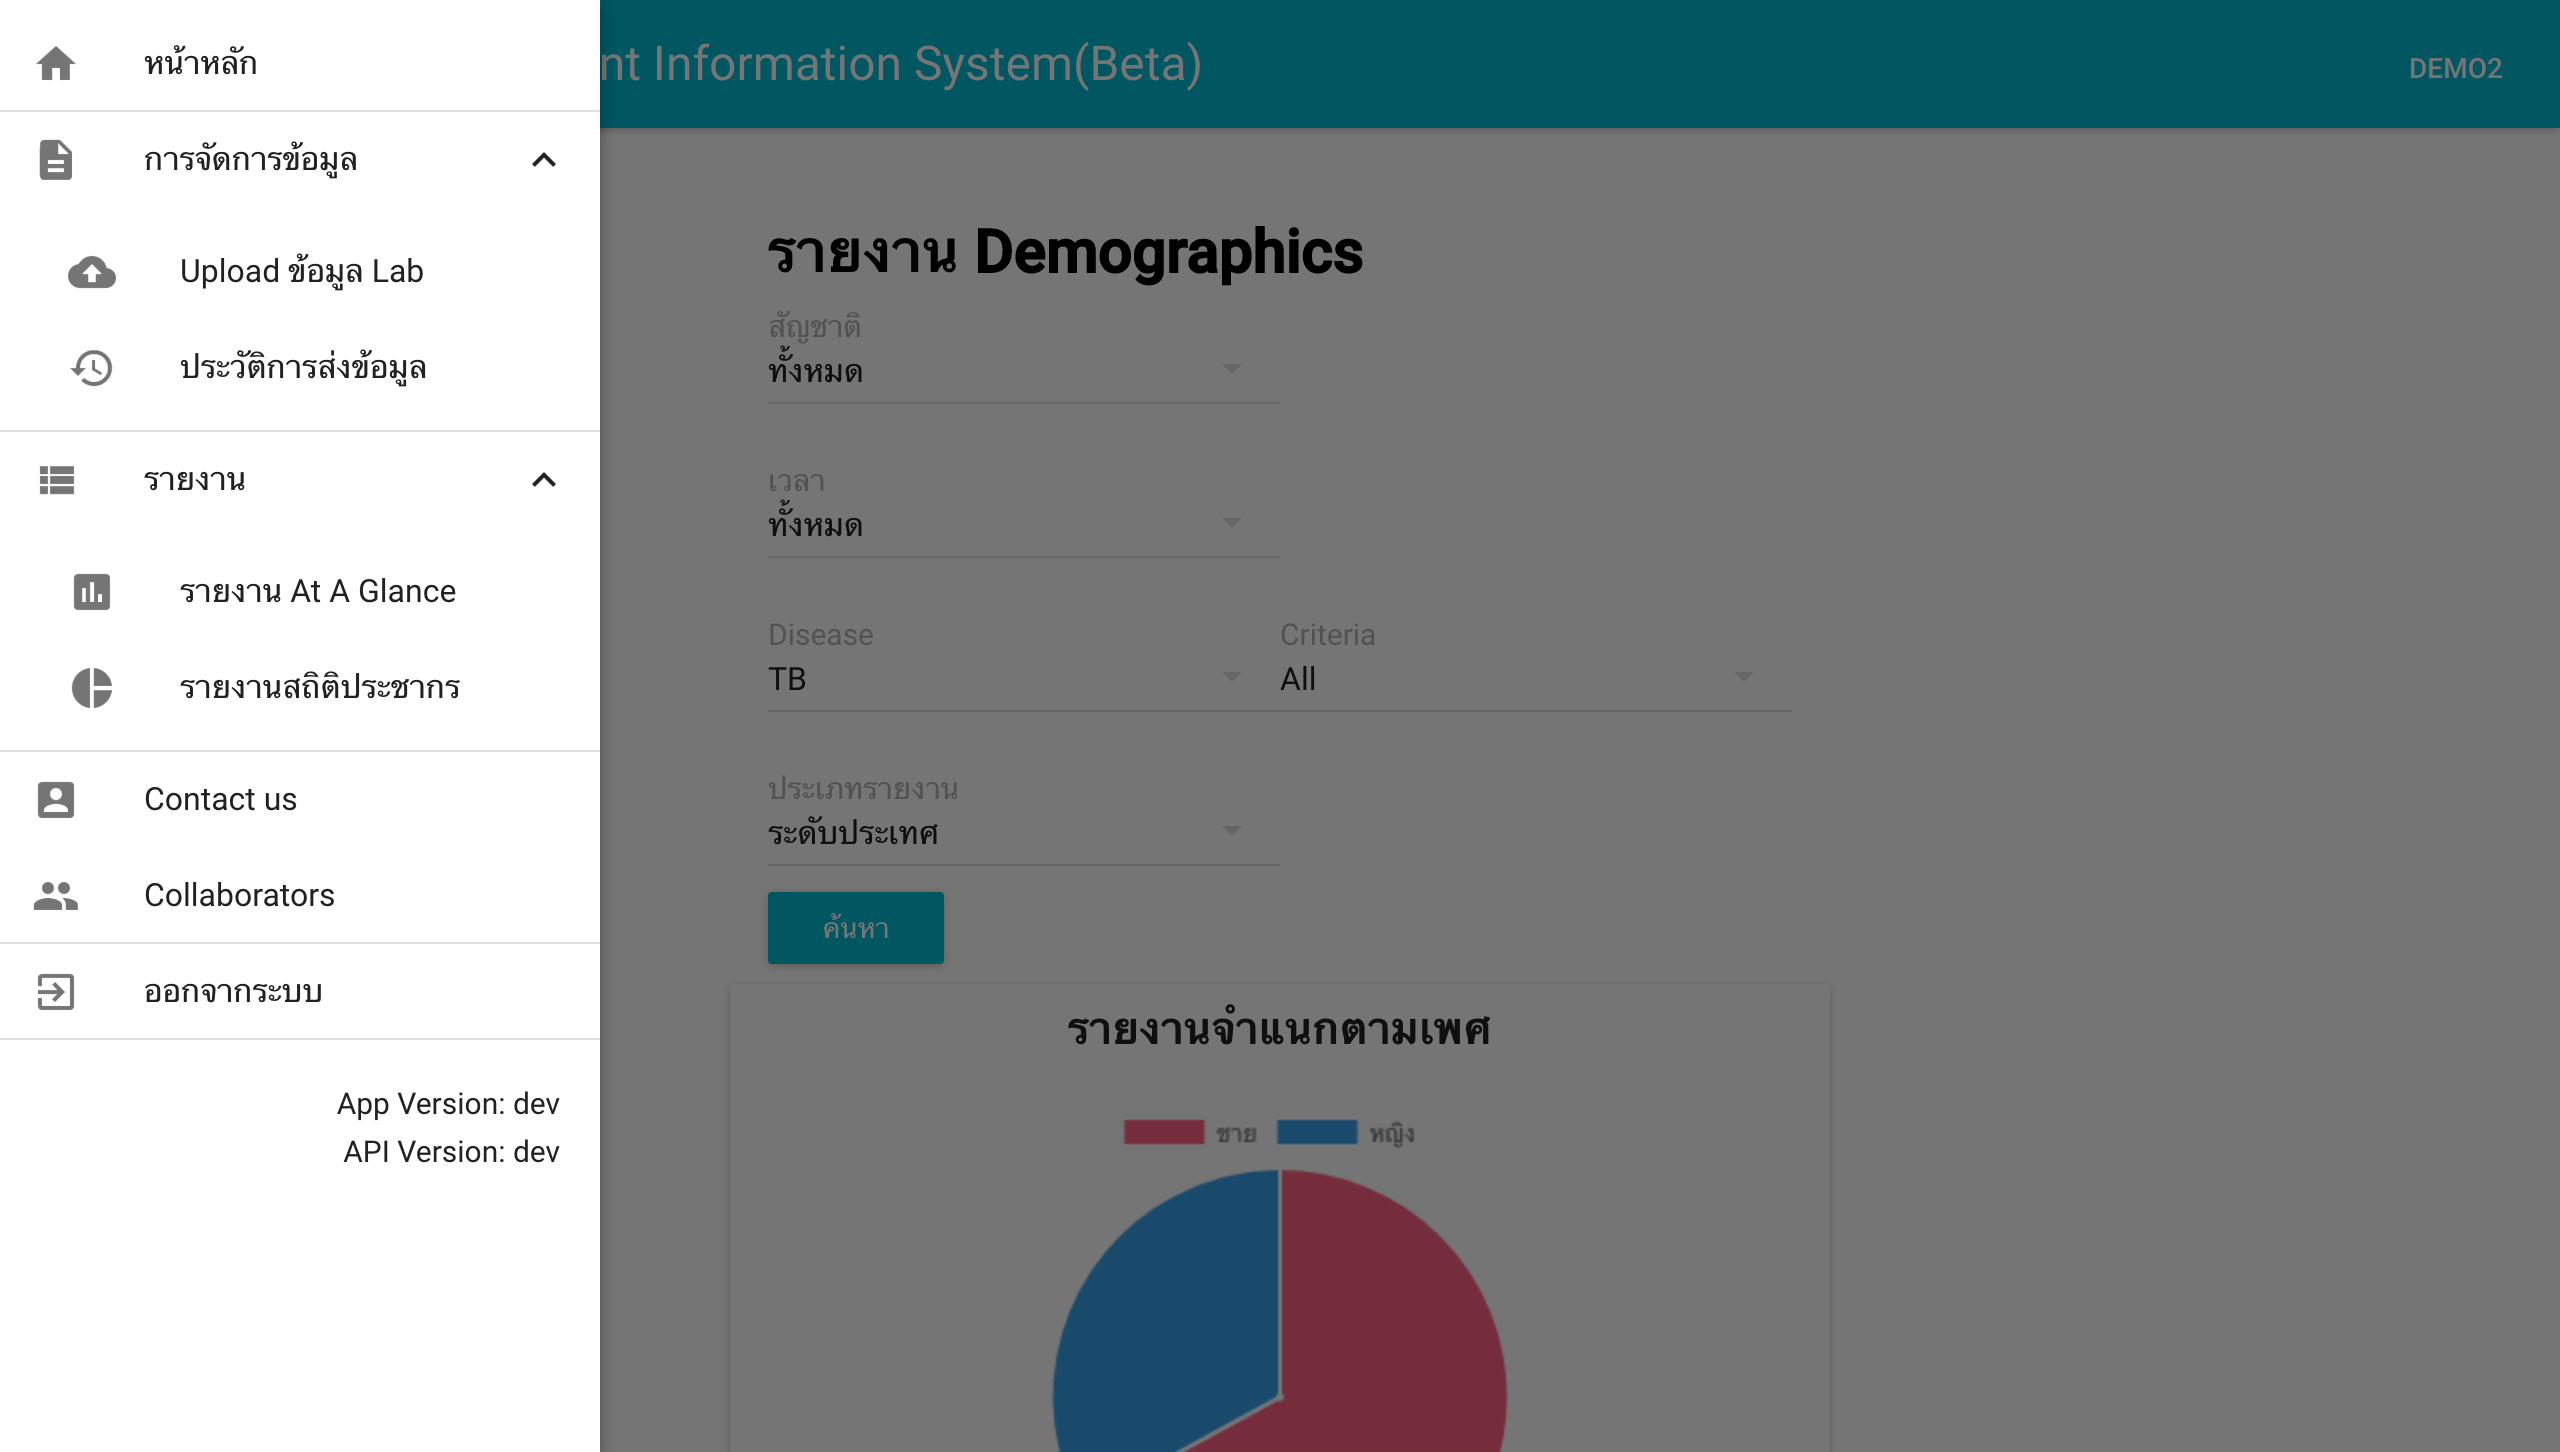
\includegraphics[width=12cm]{images/chapter-05/tab-bar-menu.png}
        		\caption{Menus}
        		\label{tab-bar-menu}
        \end{figure}
	\FloatBarrier
	
	\subsection{At a Glance Report}
	
	To see at a glance report, user need to select at a glance report in tab bar menu as shown in figure \ref{tab-bar-menu} or it will show you immediately when you log-in to the system. Then, user can select type of data that they want by selecting time, disease, criteria of the disease, and the type of report that they want. In order to see all the drop-down select, there are in section \ref{filter-data}. When user finished selecting, user need to click 'find' button as shown in figure \ref{at-a-glance-report}. Then the front-end will send the input data to the server via POST. For example, api/v1/hiv/at-a-glance/all. Then the server will send json object back, then the table will be rendered as shown in figure \ref{at-a-glance-report}. 
	
	
    \FloatBarrier
    	\begin{figure}[h!]
            \centering
                % can use width=\linewidth
        		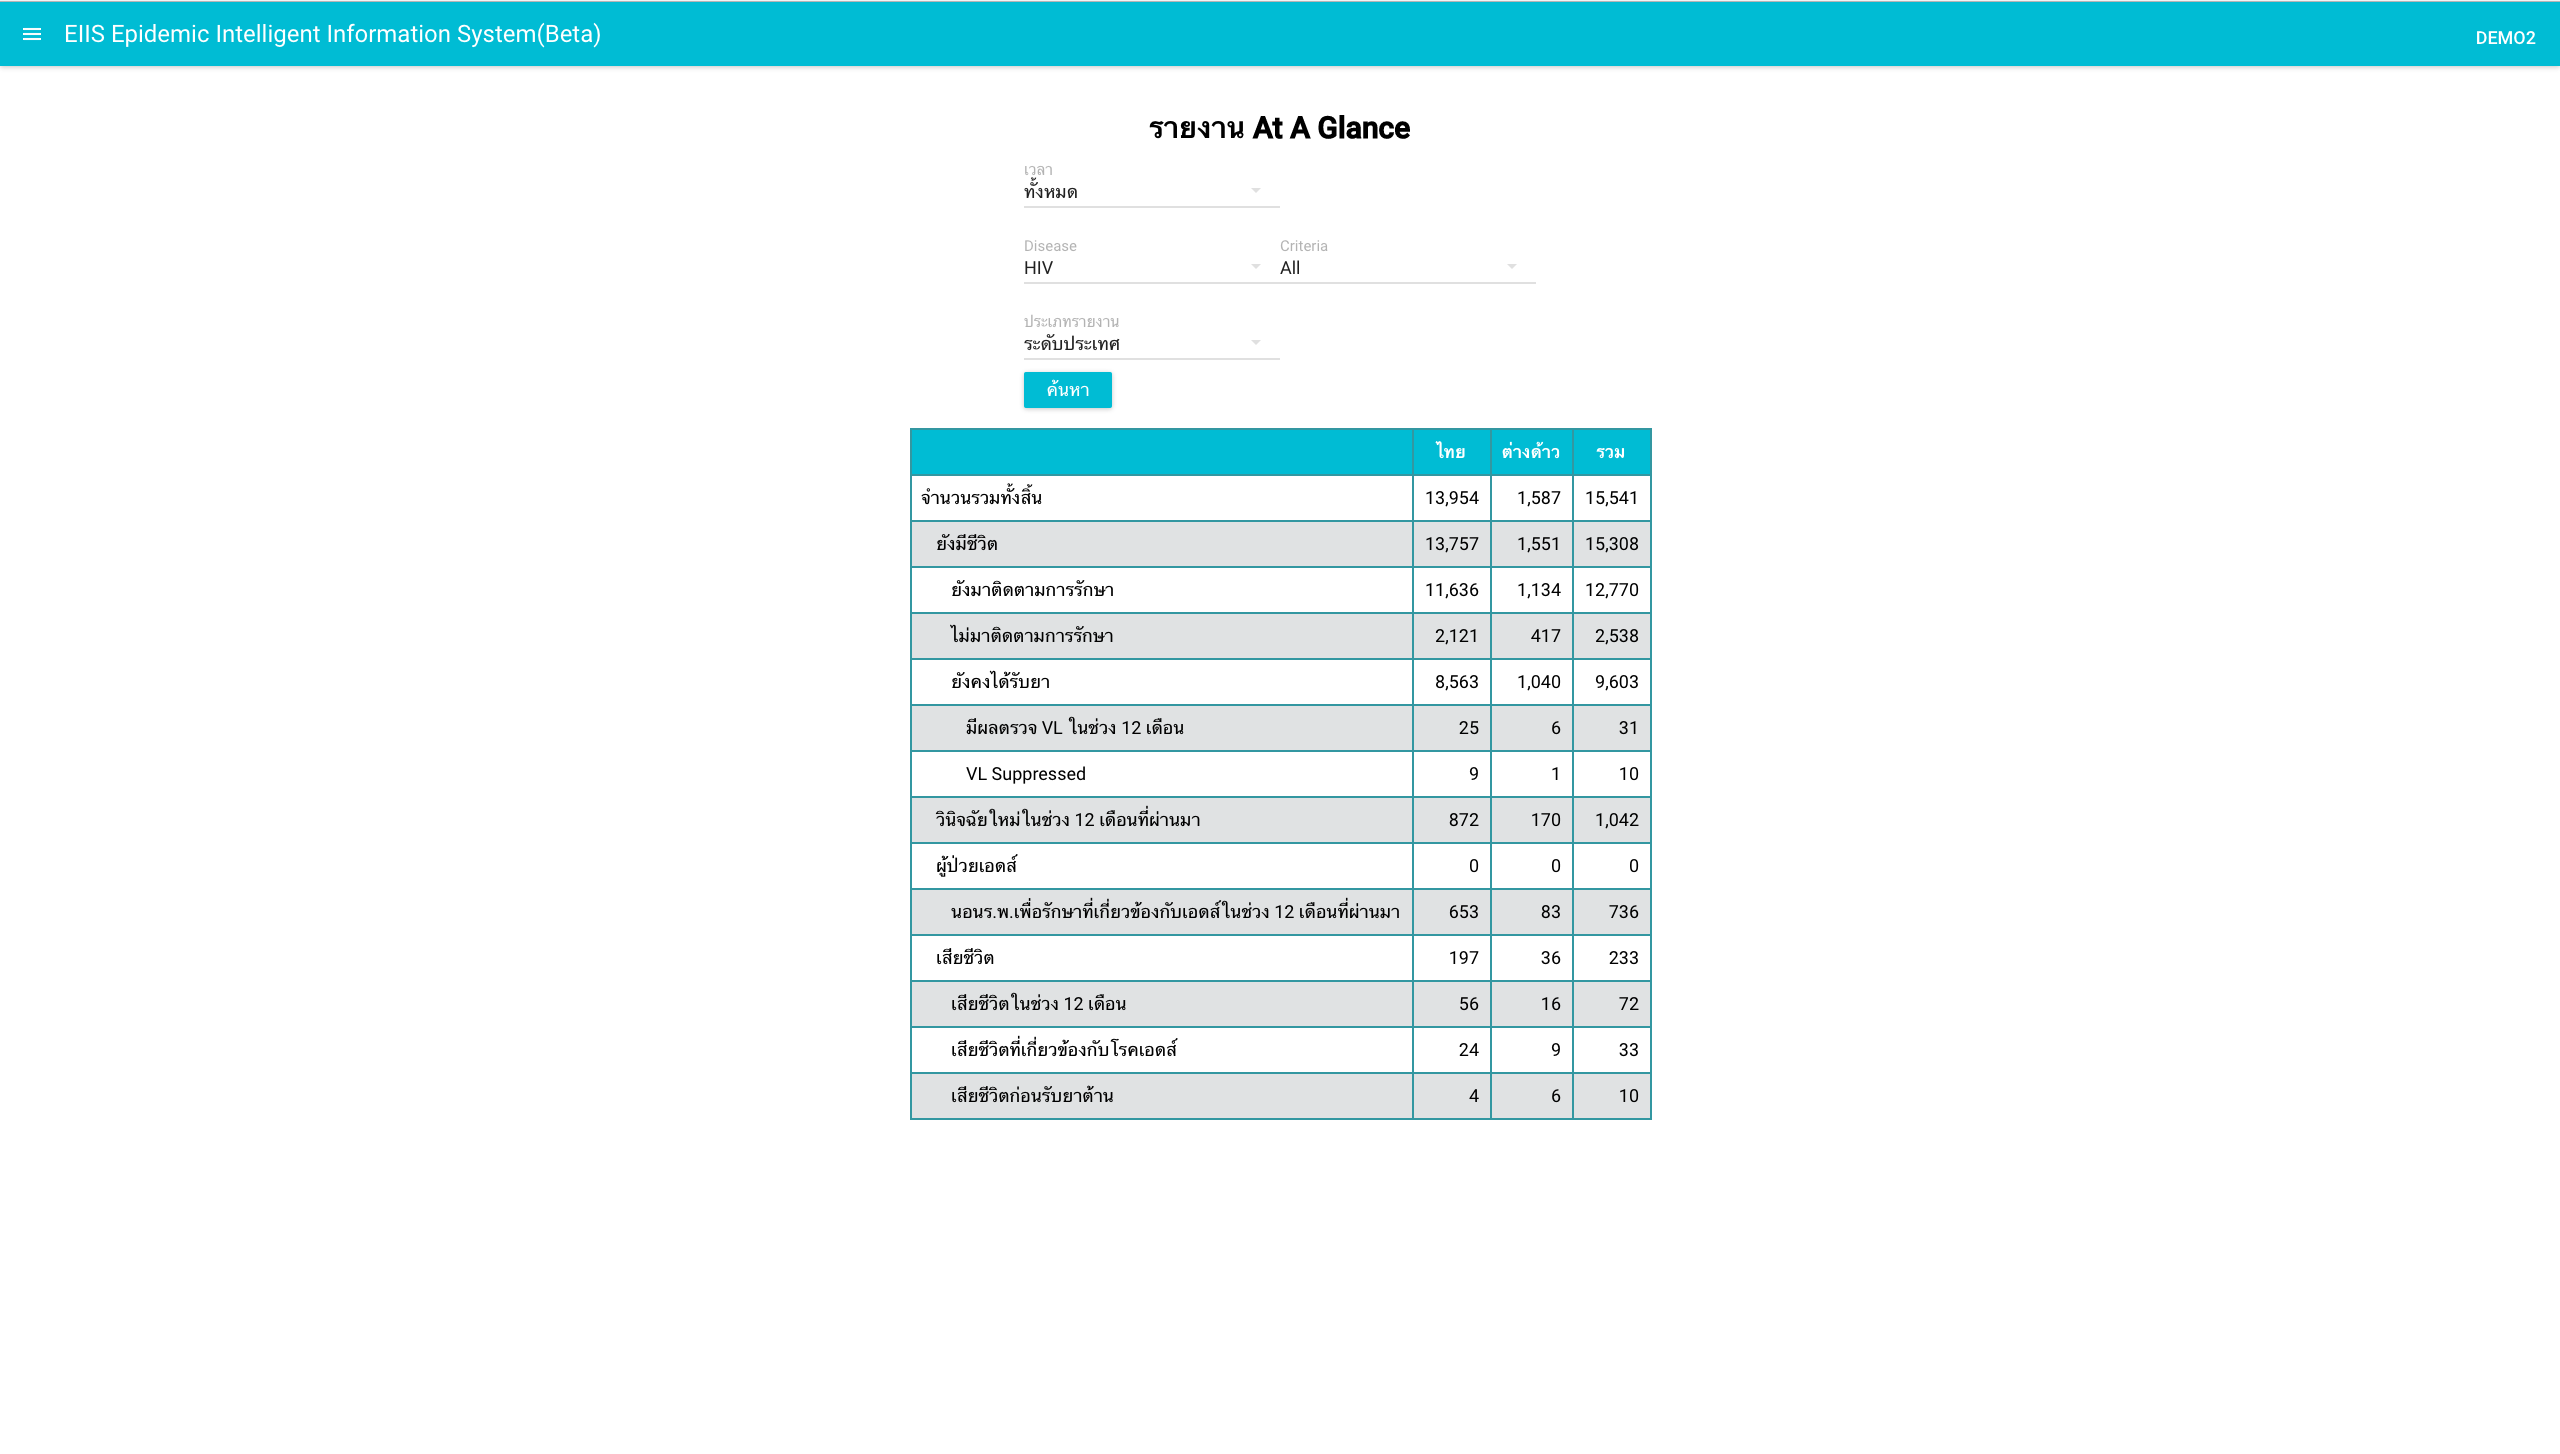
\includegraphics[width=12cm]{images/chapter-05/at-a-glance-report.png}
        		\caption{At a Glance Report}
        		\label{at-a-glance-report}
        \end{figure}
	\FloatBarrier
	

	
	\subsection{Upload File} \label{upload_file}
	To upload file to EIIS application, user need to select upload lab file in tab bar menu that shown in figure \ref{tab-bar-menu}. Then, user need to select hospital(it will be provides according to the role of that user), month, and year as in figure \ref{upload-status1} then click next to go to another step. In step two, user need to select the file, either file-in or file-out, but at least user need to pick one file in order to upload then click upload button as shown in figure \ref{upload-status2}. After that the front-end will send the data with POST method. For instance, /api/v1/extralab/upload. Next, the server will send the data back to the front-end and shows the data as shown in figure \ref{upload-status3}. In addition, if user do not put any file and click upload button, the upload box will be red ,as shown in figure \ref{upload-error},as warning the user that they have to put some file in order to upload.
   	
   	\vspace{10mm}
    \FloatBarrier
    	\begin{figure}[h!]
            \centering
                % can use width=\linewidth
        		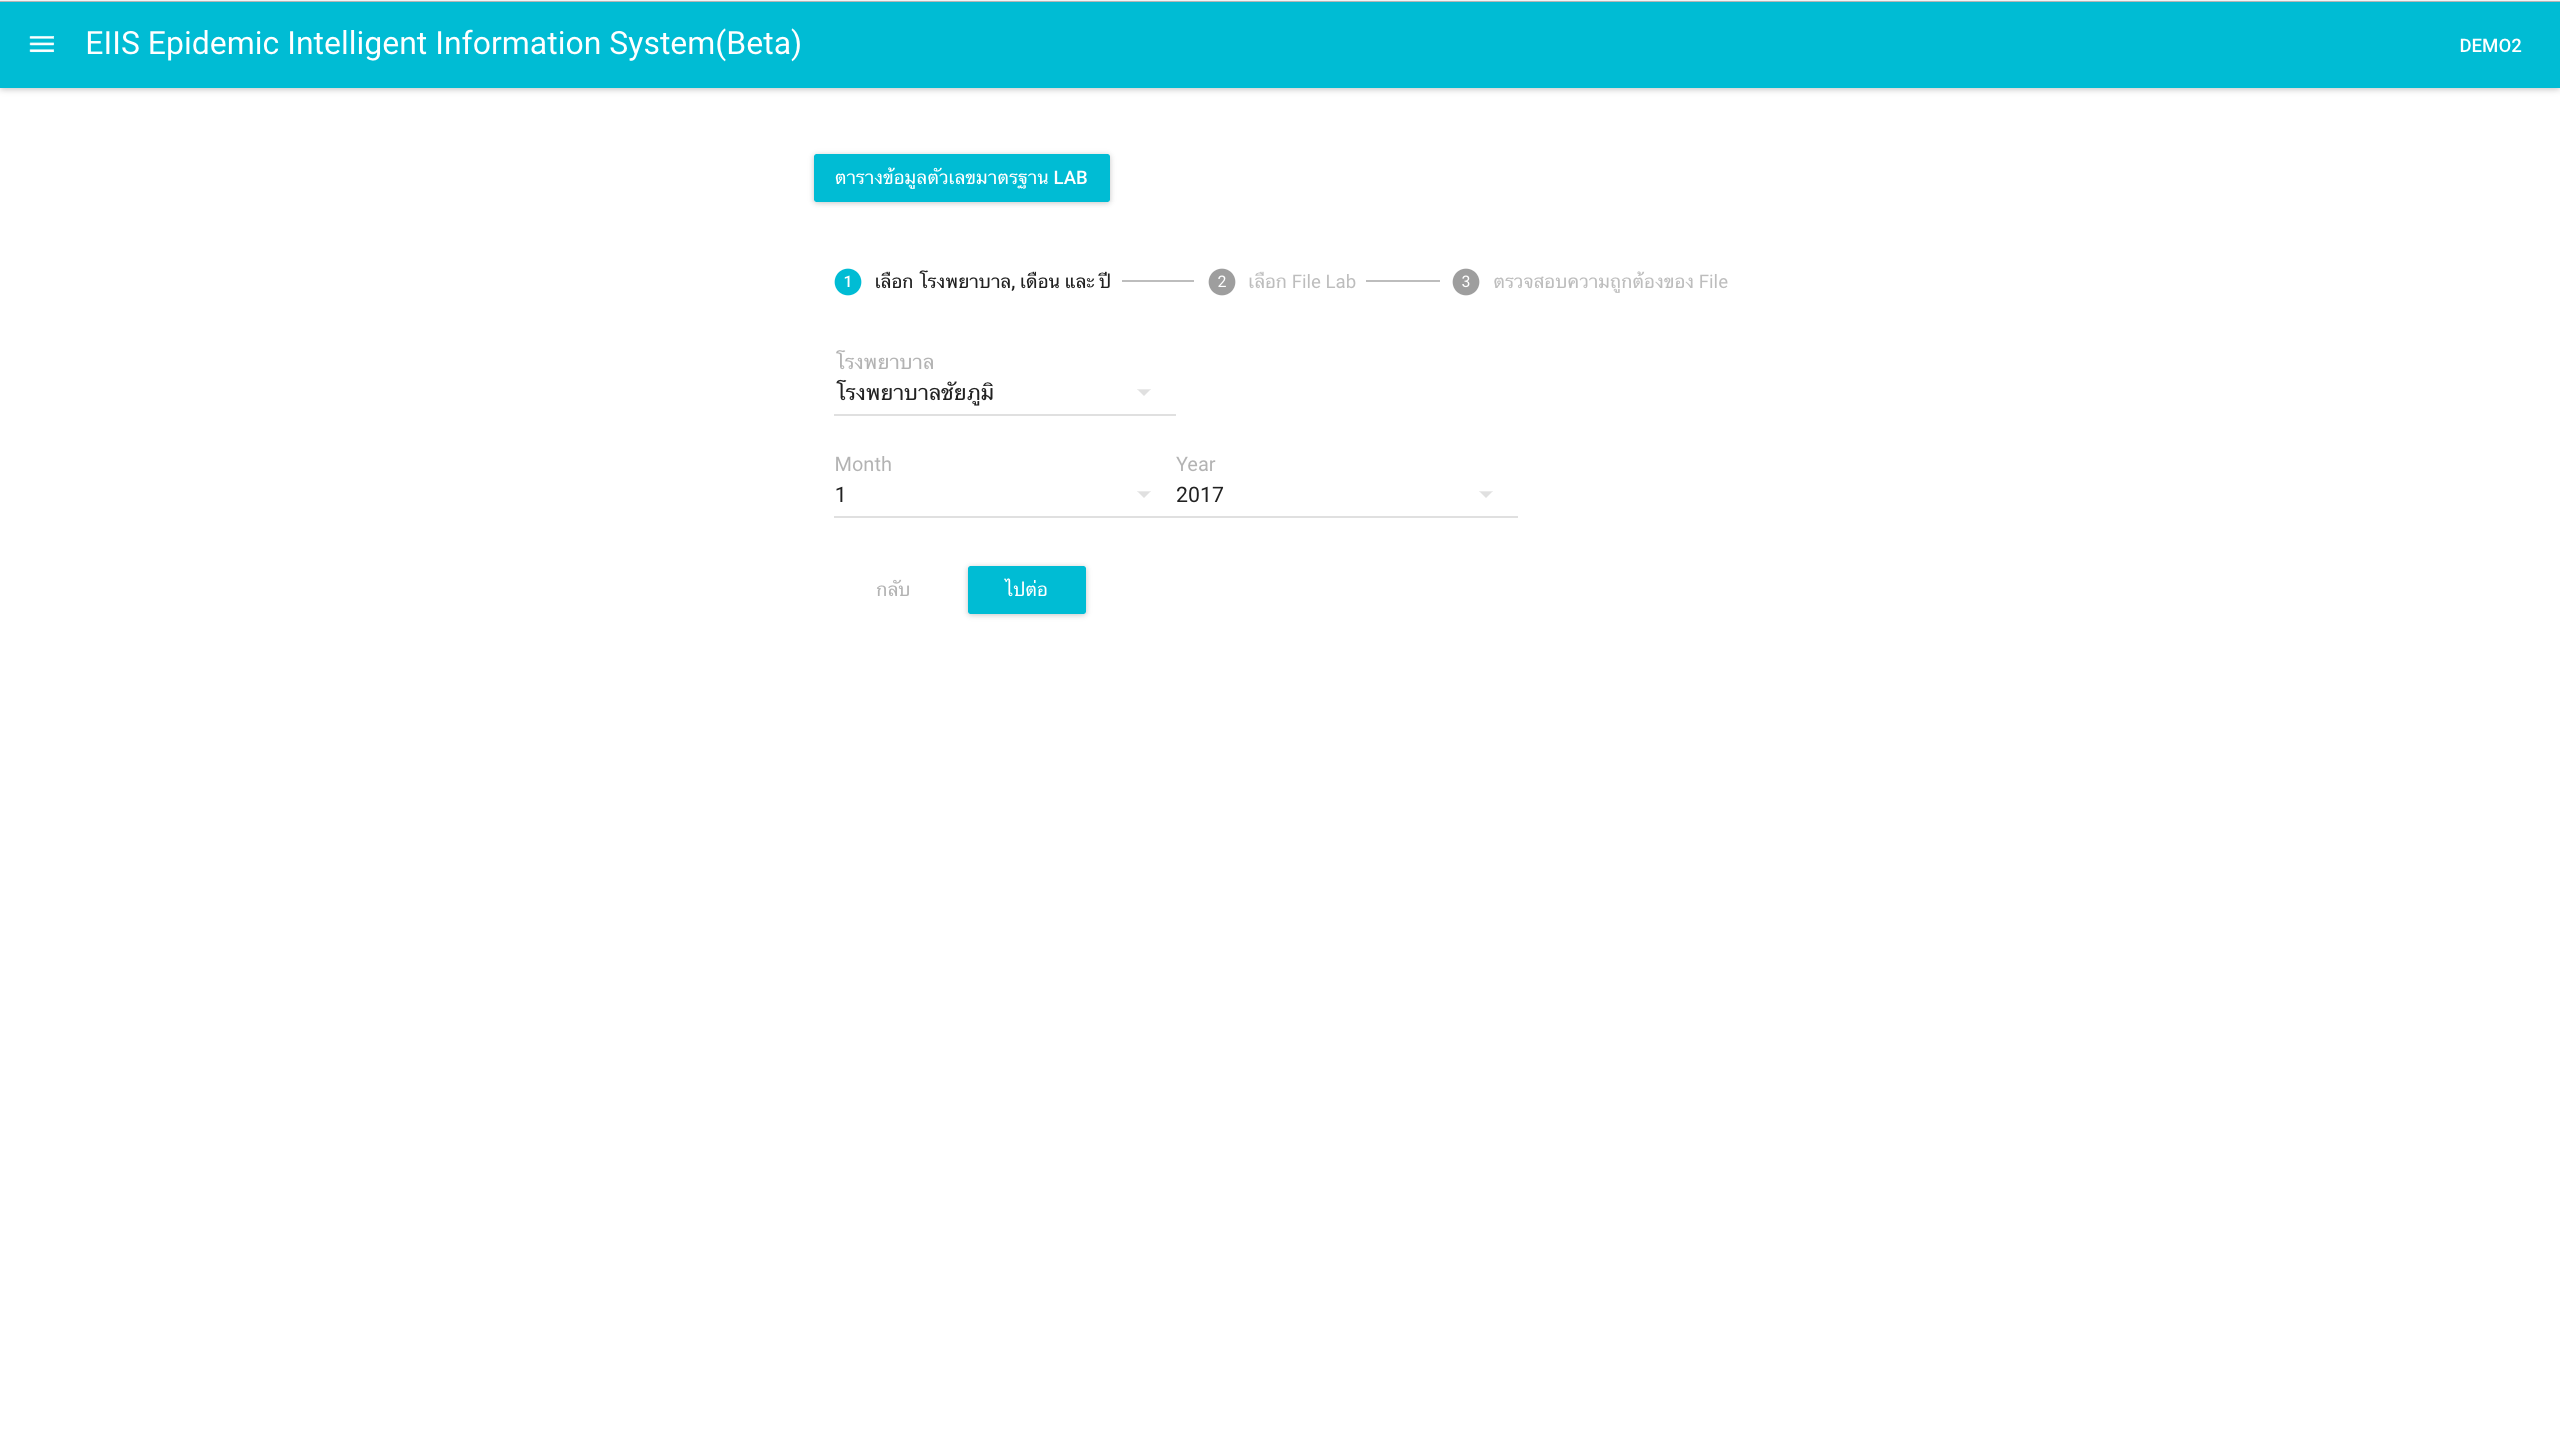
\includegraphics[width=12cm]{images/chapter-05/upload1.png}
        		\caption{Uploading lab file page when user selecting hospital, month, and year}
        		\label{upload-status1}
        \end{figure}
	\FloatBarrier
	
	\FloatBarrier
    	\begin{figure}[h!]
            \centering
                % can use width=\linewidth
        		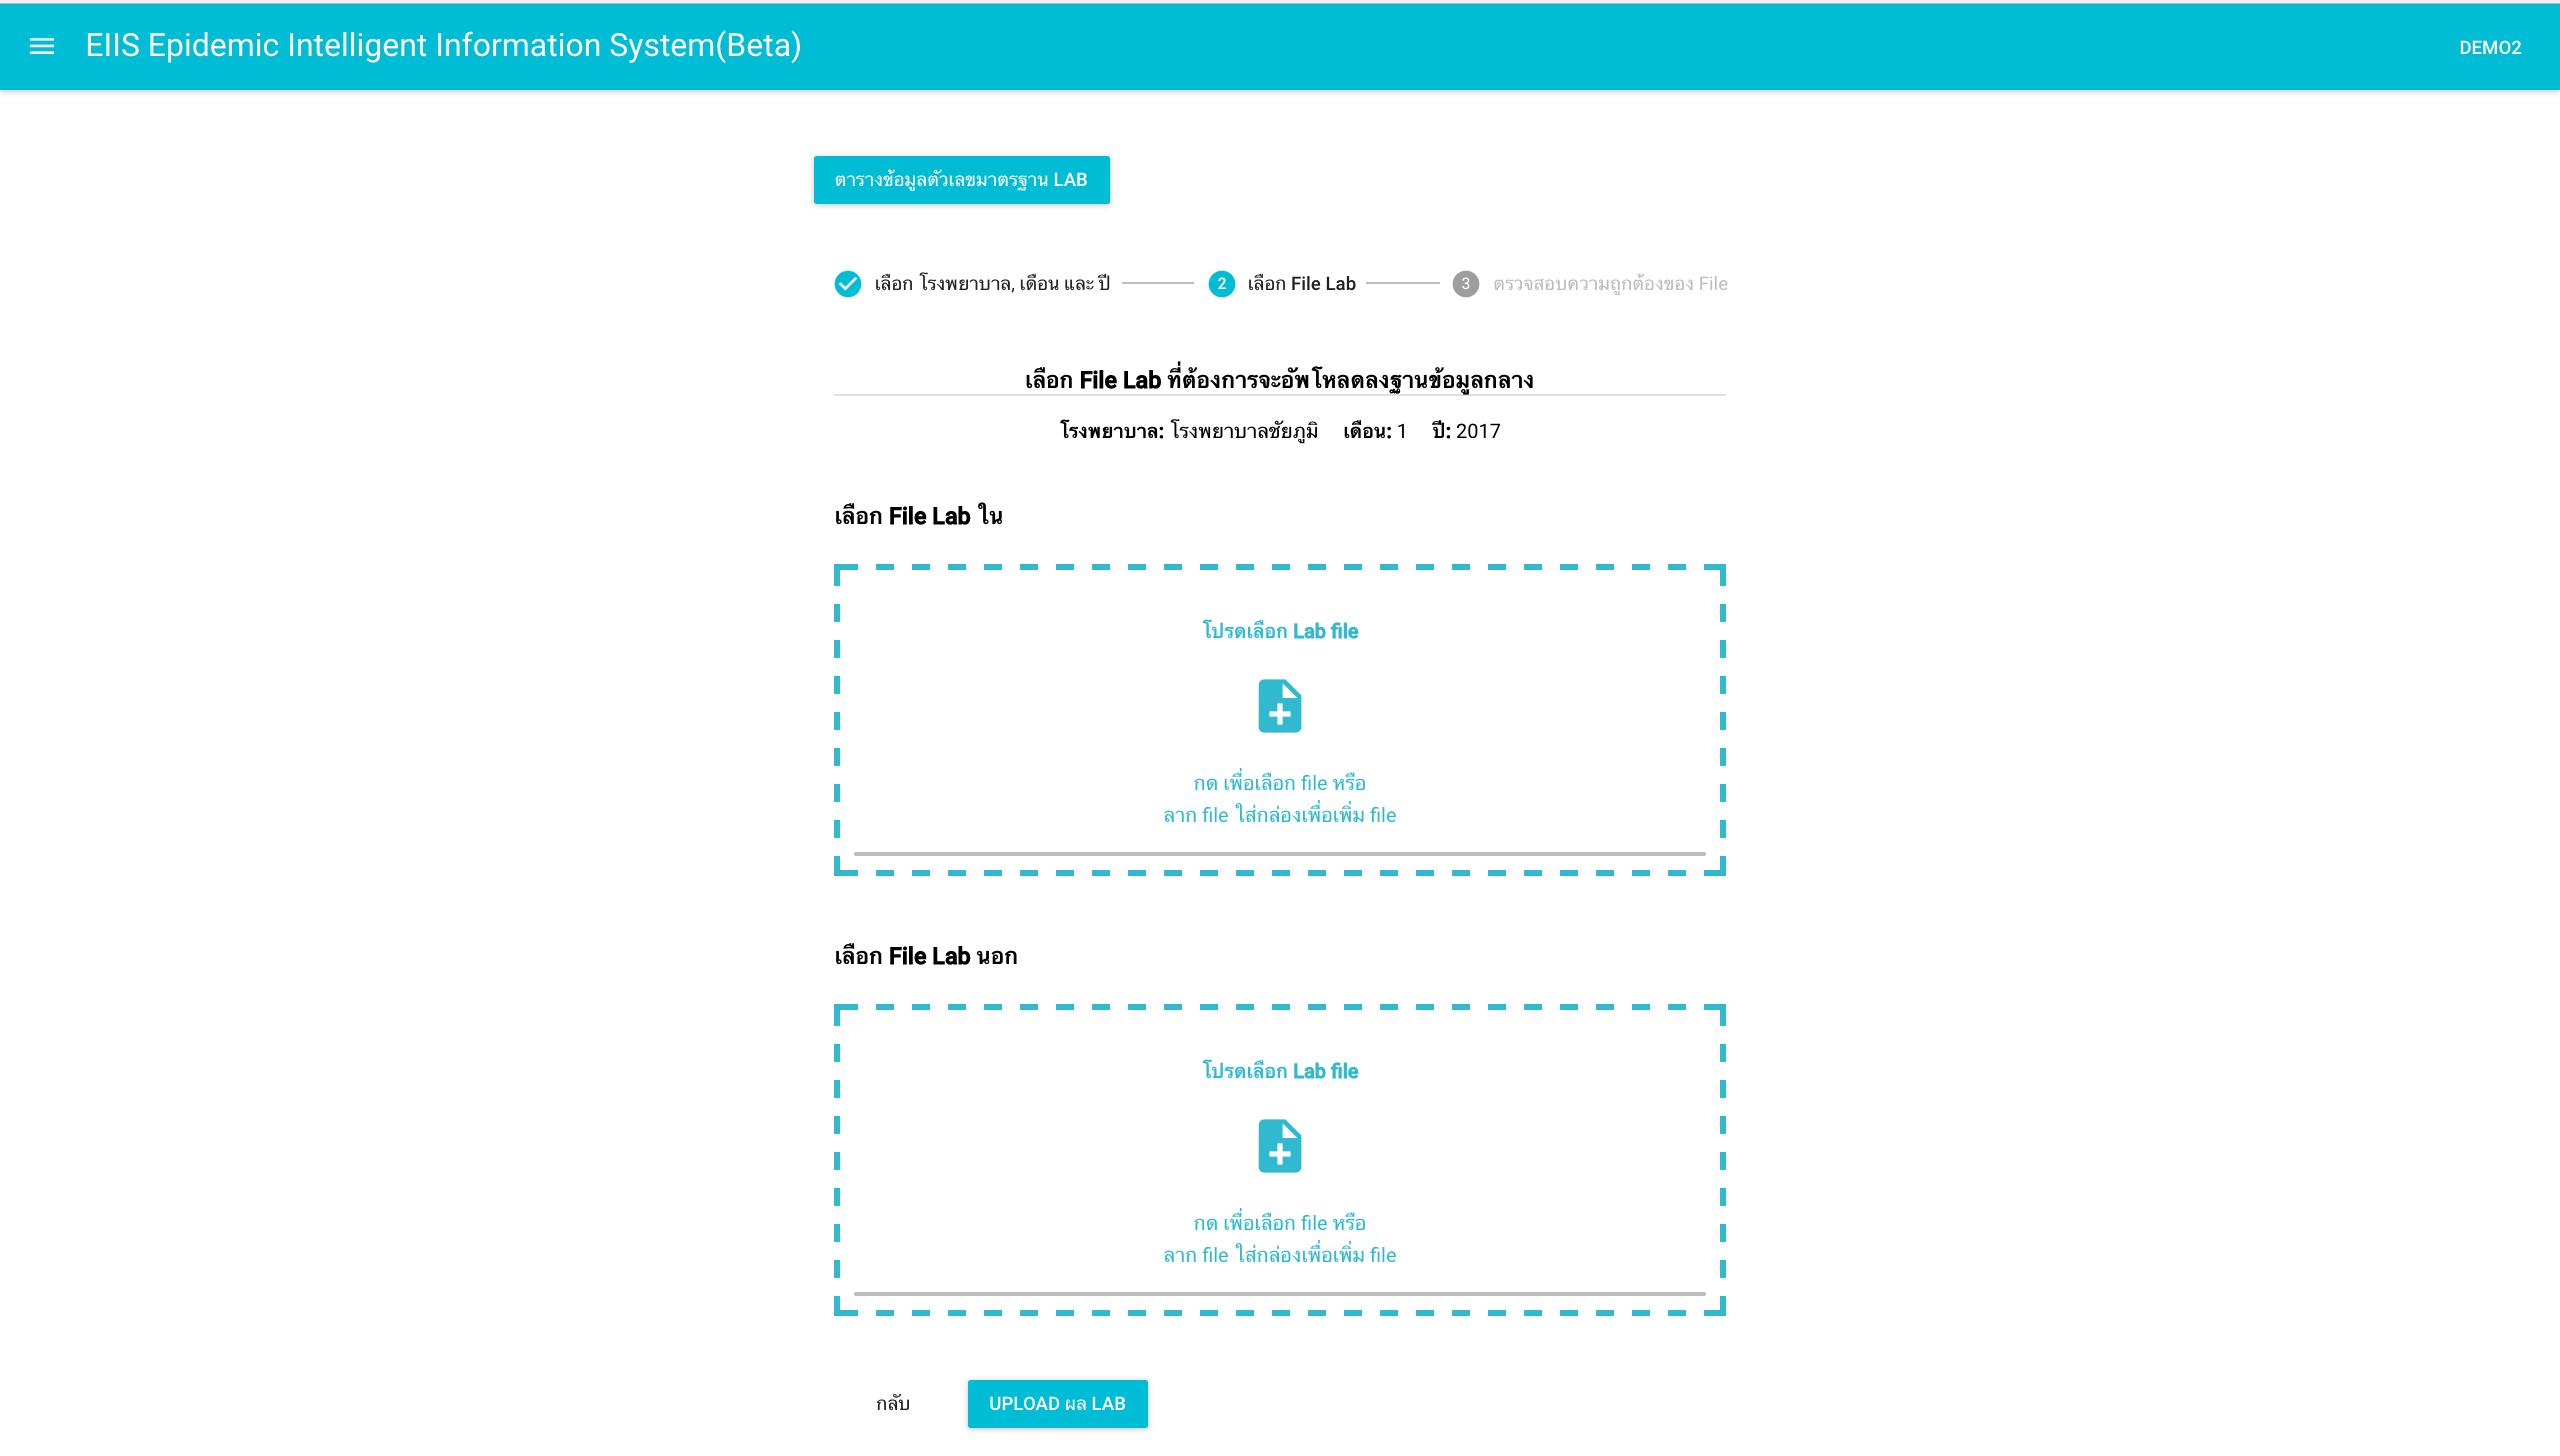
\includegraphics[width=12cm]{images/chapter-05/upload2.png}
        		\caption{Uploading lab file page when user uploading in-patient lab file or out-patien lab file}
        		\label{upload-status2}
        \end{figure}
	\FloatBarrier
	
	\FloatBarrier
    	\begin{figure}[h!]
            \centering
                % can use width=\linewidth
        		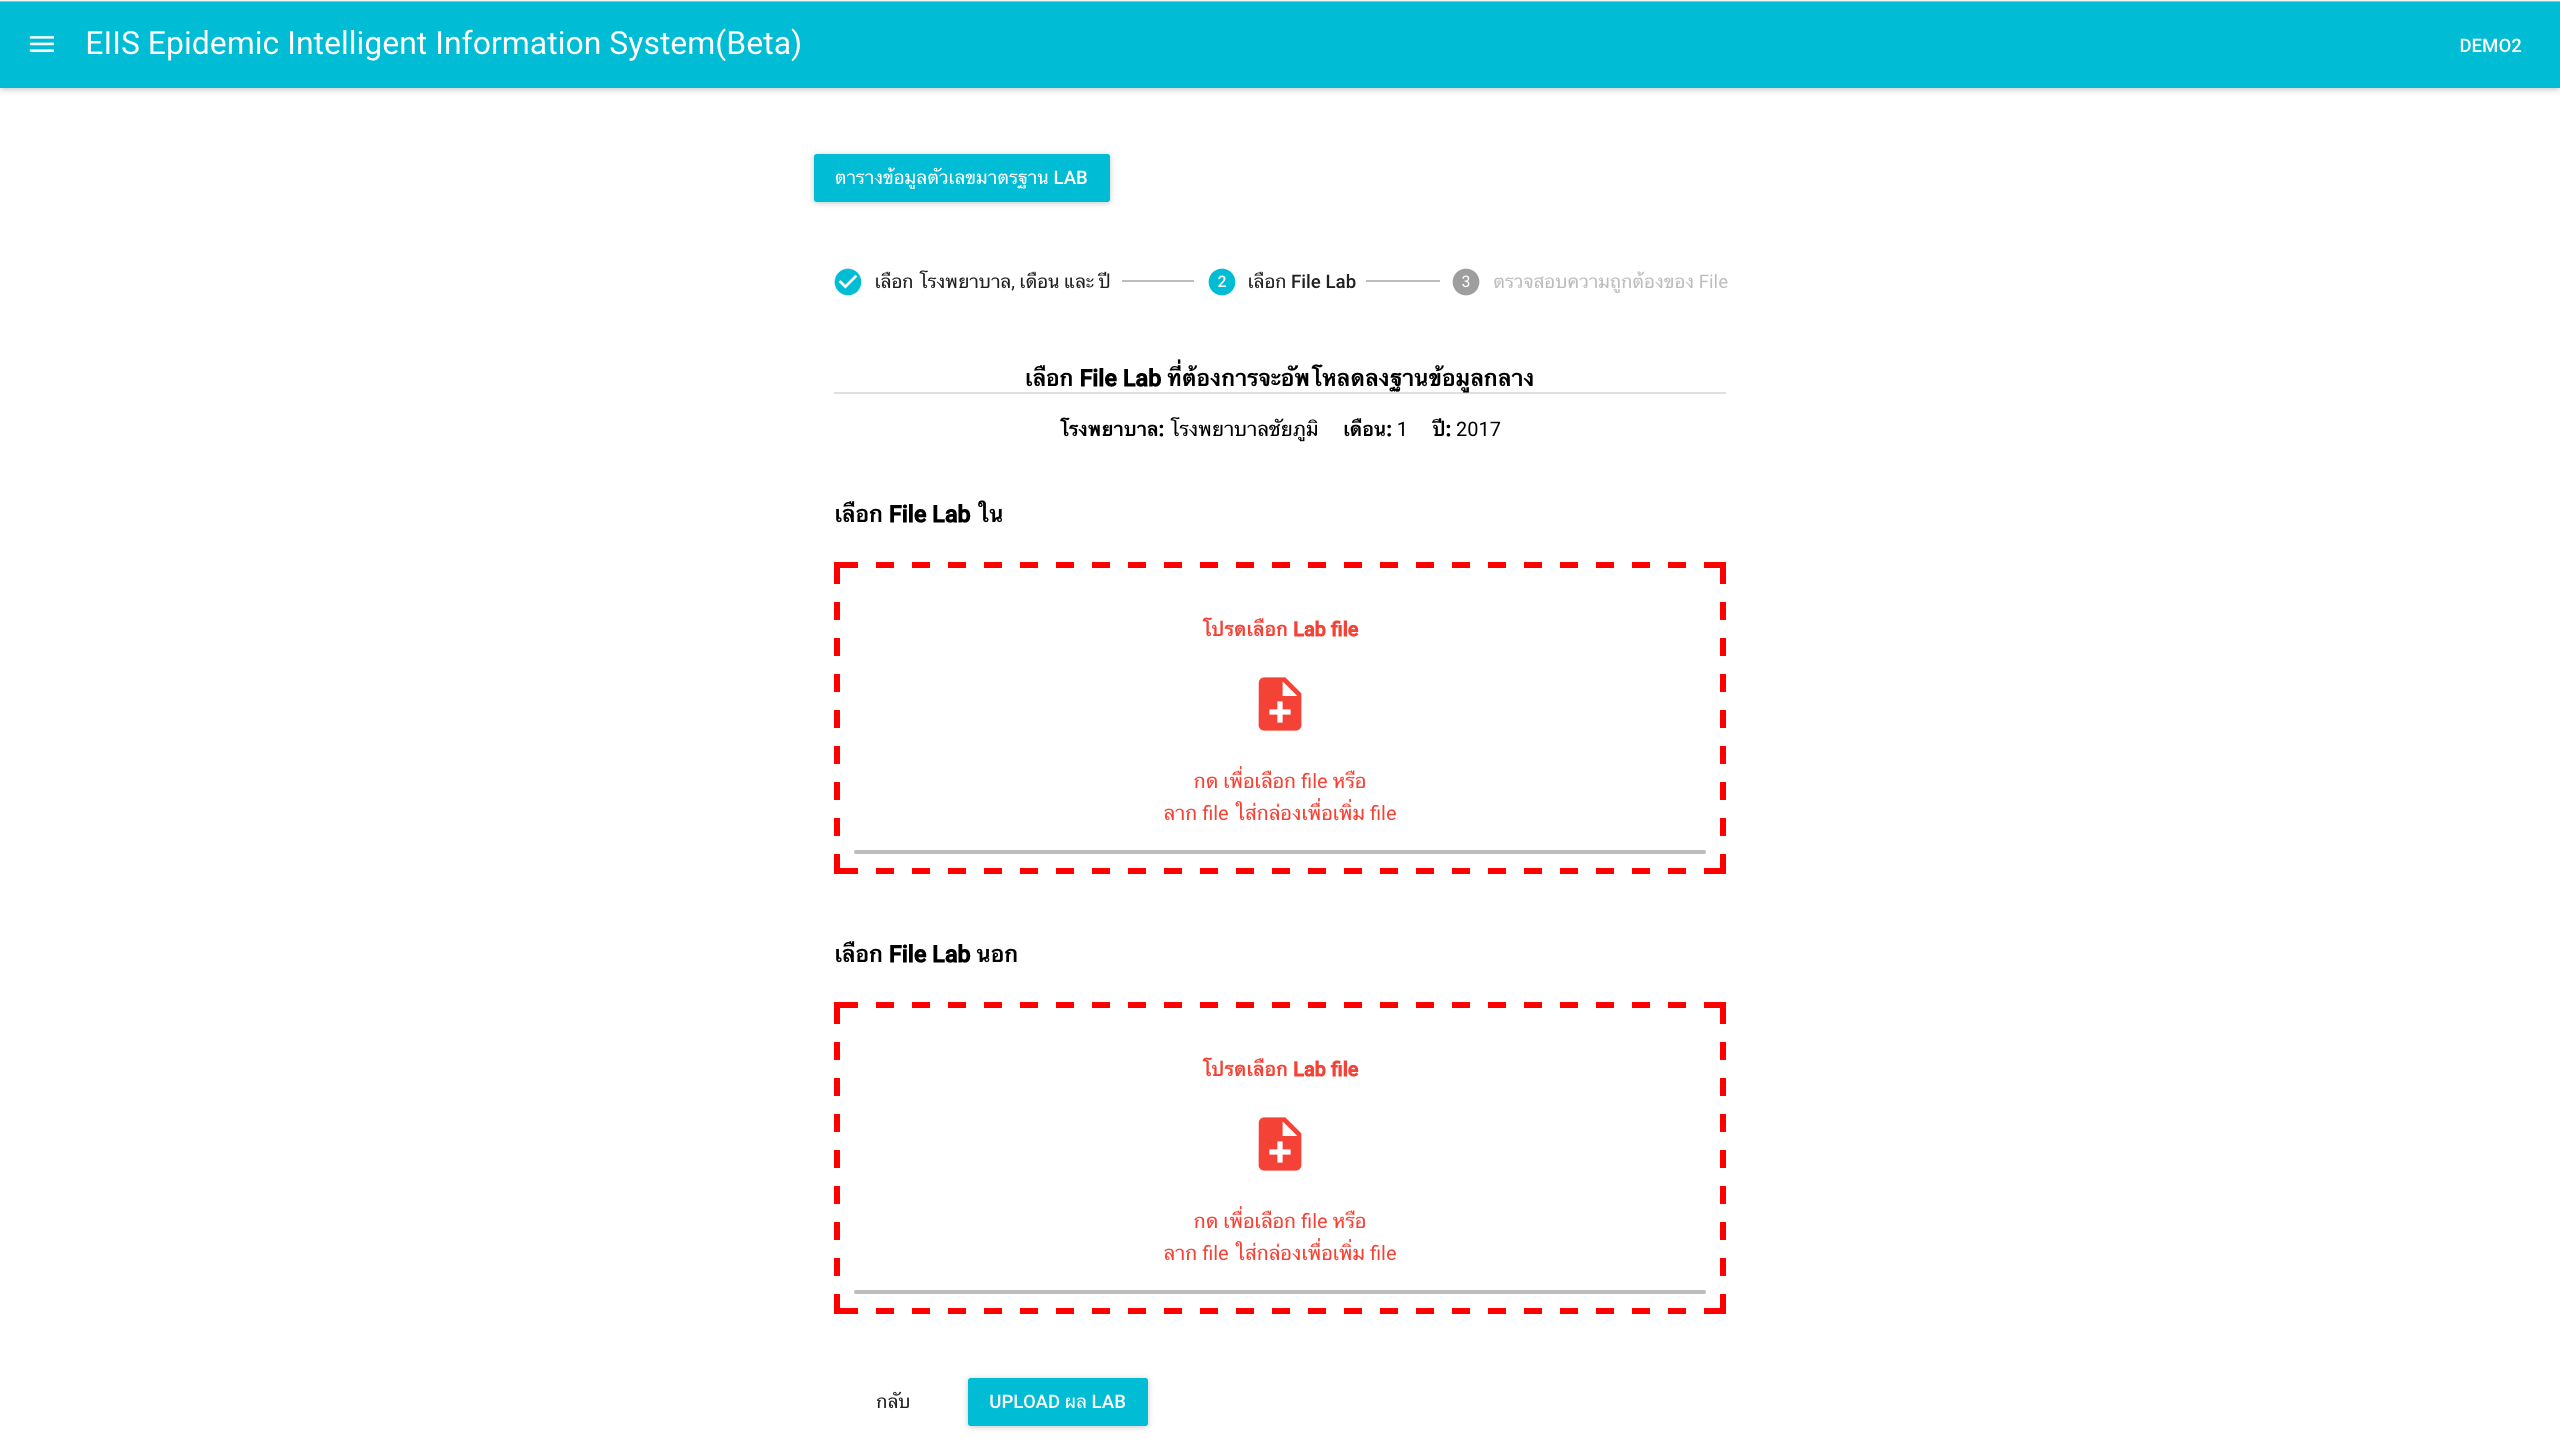
\includegraphics[width=12cm]{images/chapter-05/upload-error.png}
        		% \caption{Upload Error}
        		\caption{Red highlight indicating that the user must select the lab file for uploading to the system}
        		\label{upload-error}
        \end{figure}
	\FloatBarrier
	
	\FloatBarrier
    	\begin{figure}[h!]
            \centering
                % can use width=\linewidth
        		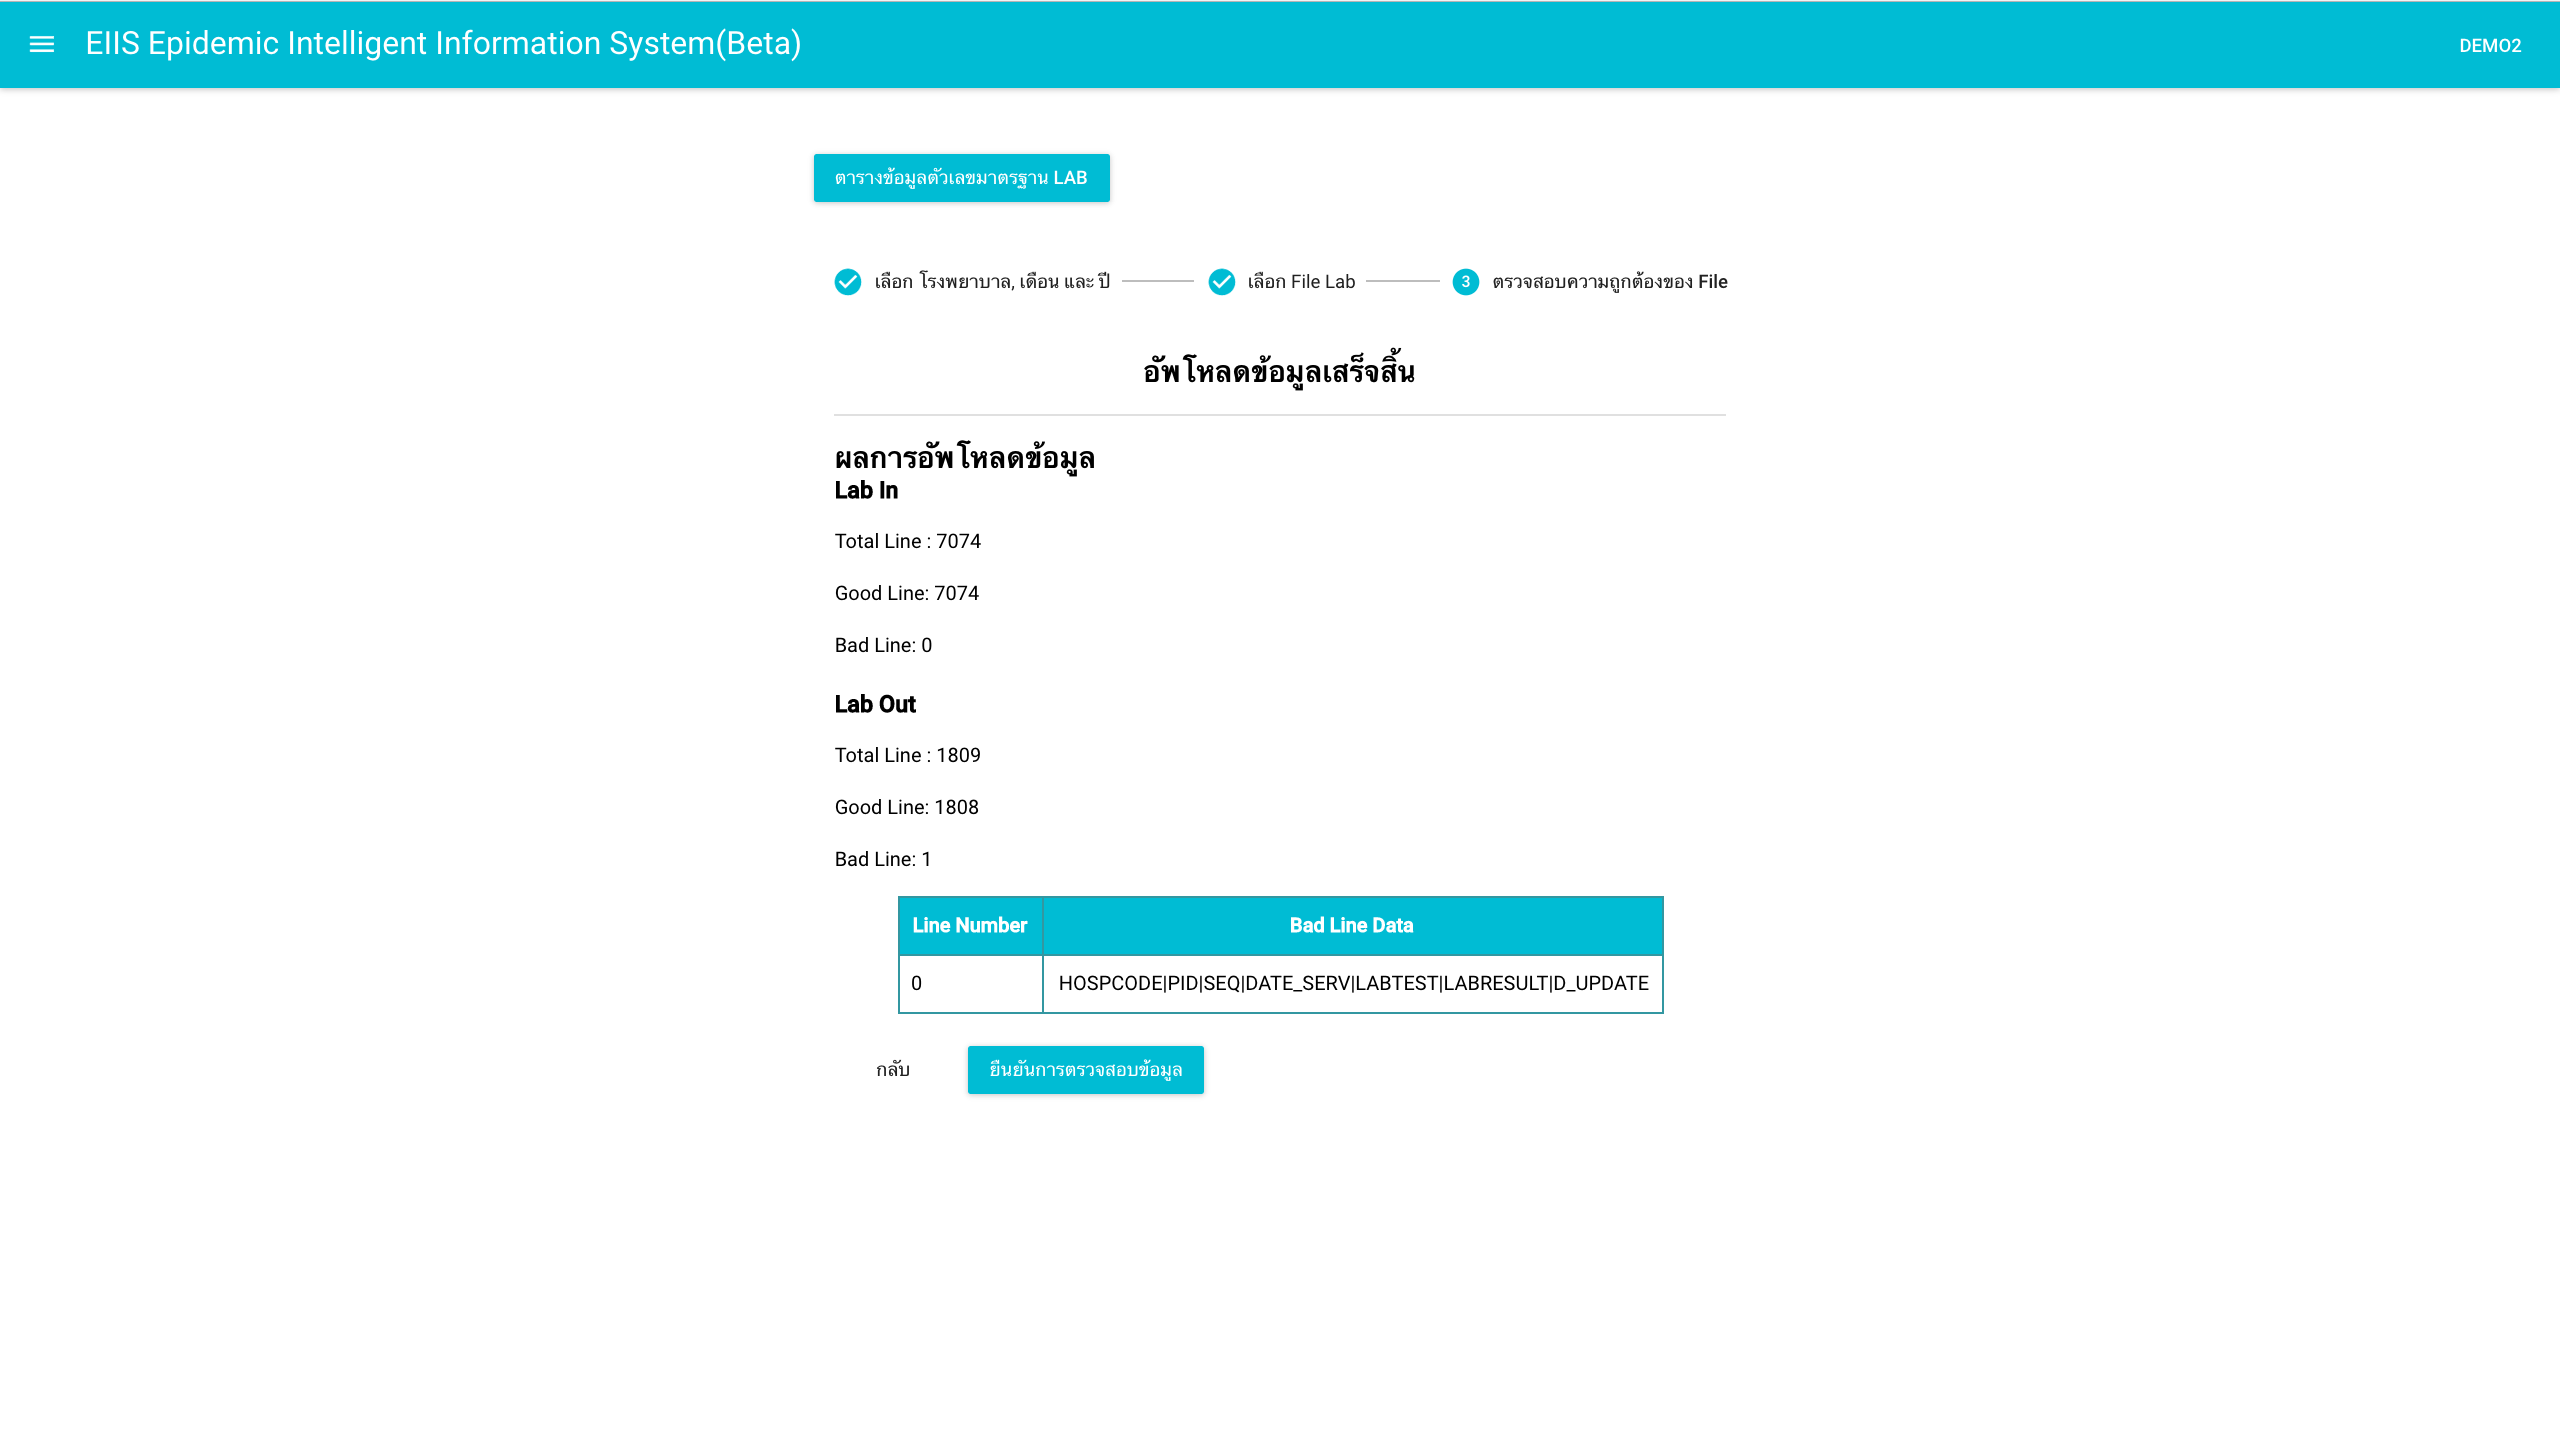
\includegraphics[width=12cm]{images/chapter-05/upload3.png}
        		\caption{Result after user uploading lab file(s)}
        		\label{upload-status3}
        \end{figure}
	\FloatBarrier
	
	
	\subsection{Checking Upload History Status} \label{check_upload_history_status_ui}
% 	/api/v1/extralab/check-status 
	
	To check upload status,user need to select check history of upload file in tab bar menu that shown in figure \ref{tab-bar-menu}. Then, user can select type of report, area, province, and year that they want. In order to see all the drop-down select, there are in section \ref{filter-data}. When user finished selecting, user need to click 'find' button as shown in figure \ref{upload-status0}. The front-end will send the input data to the server via POST. For example, /api/v1/extralab/check-status. After that the server will send json object back, and the table will be rendered as shown in figure \ref{upload-status}. 
	
    \FloatBarrier
    	\begin{figure}[h!]
            \centering
                % can use width=\linewidth
        		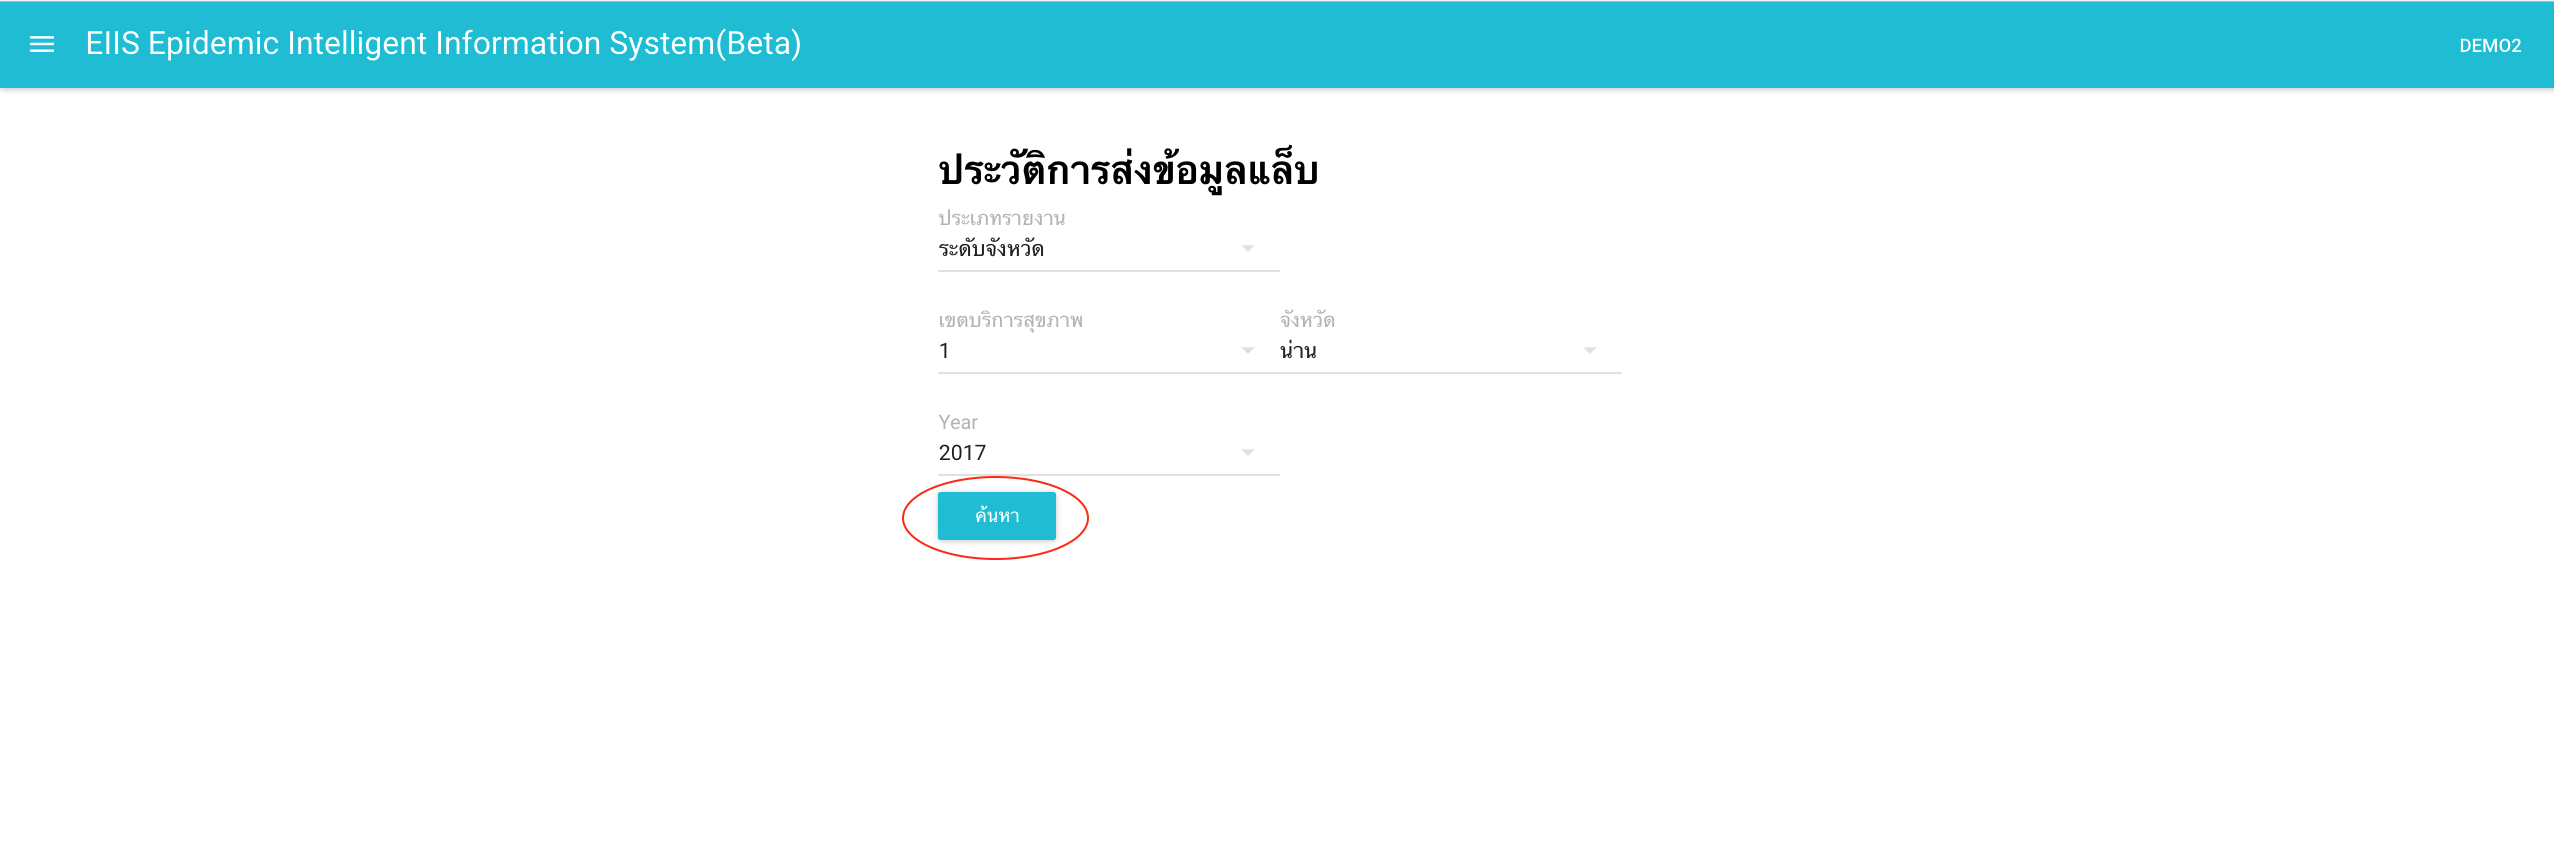
\includegraphics[width=12cm]{images/chapter-05/check-upload-status0.png}
        		\caption{Checking uploaded lab files status}
        		\label{upload-status0}
        \end{figure}
	\FloatBarrier
	
	\FloatBarrier
    	\begin{figure}[h!]
            \centering
                % can use width=\linewidth
        		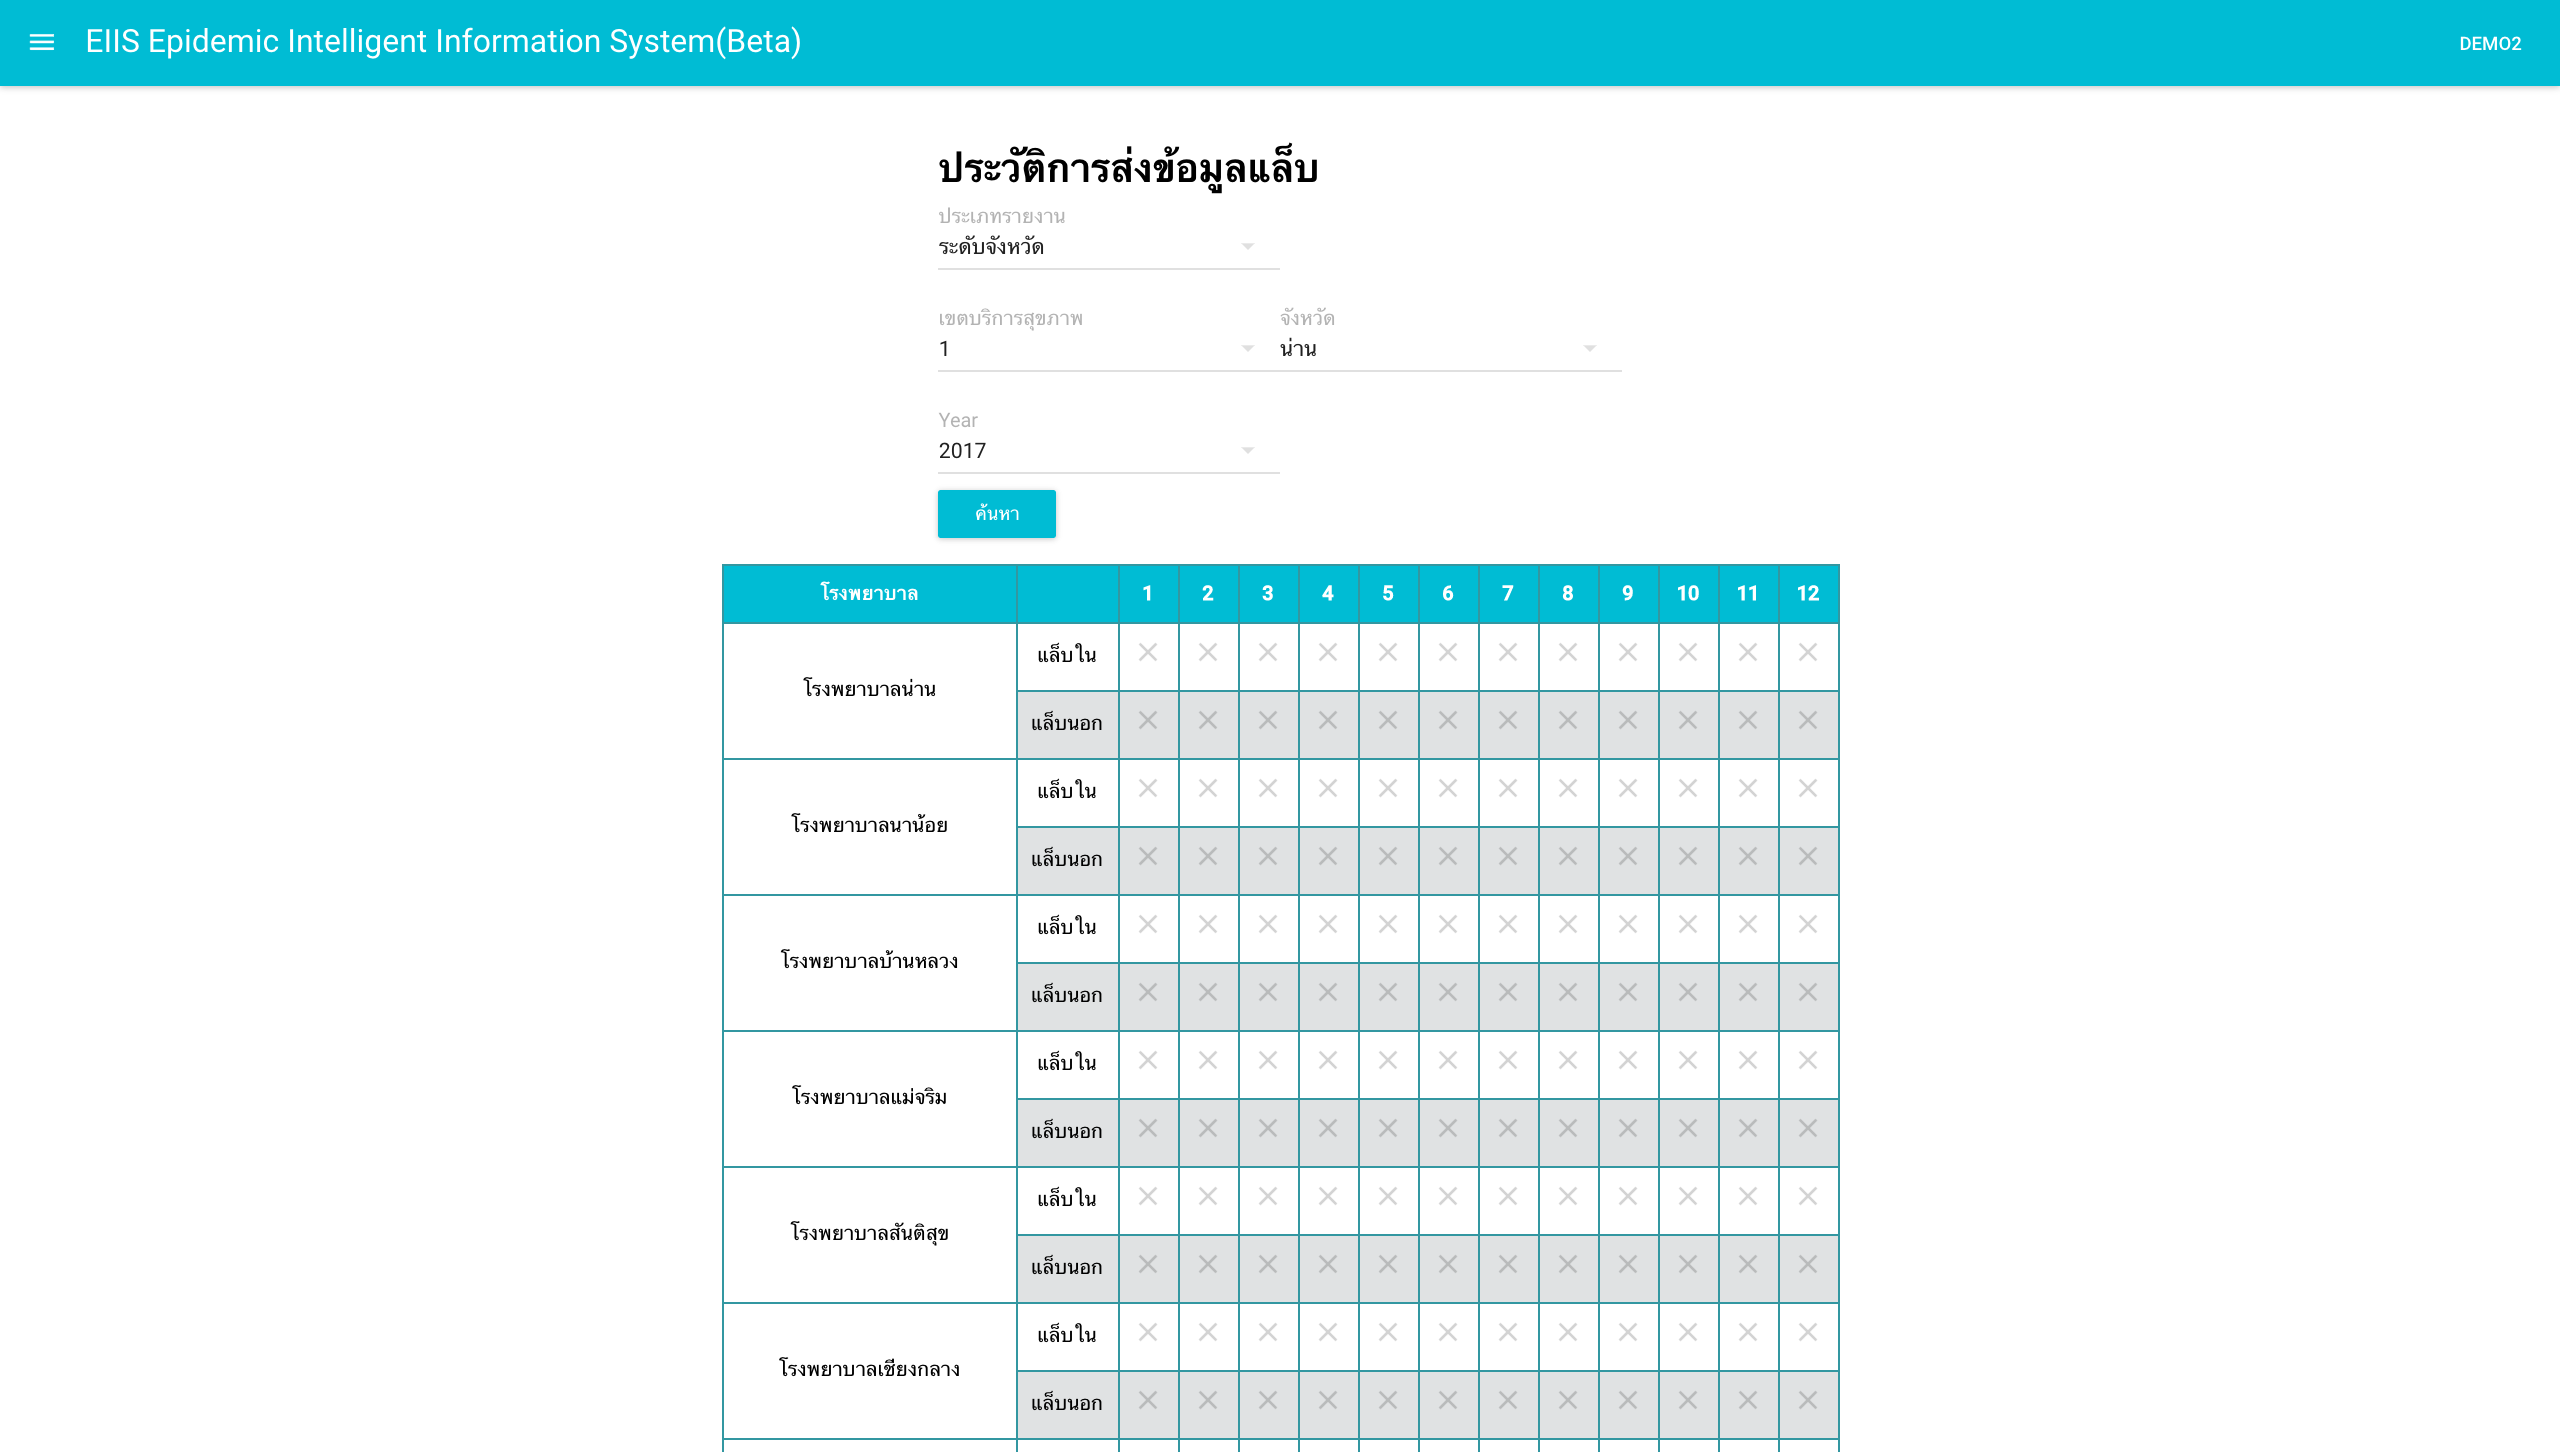
\includegraphics[width=12cm]{images/chapter-05/check-upload-status.png}
        		\caption{Status of uploaded lab files from hospitals in a region}
        		\label{upload-status}
        \end{figure}
	\FloatBarrier
	
	
	\subsection{Demographics Report} \label{demographics_report}
	
	To see at a demographics report,user need to select demographics report in tab bar menu that shown in figure \ref{tab-bar-menu}. Then, user can select type of data that they want by selecting nation, time, disease, criteria of the disease, and the type of report that they want. In order to see all the drop-down select, there are in section \ref{filter-data}. When user finished selecting, user need to click 'find' button as shown in figure \ref{demographics-report}. Then the front-end will send the input data to the server via POST. For example, /api/v1/hiv/demographic/all. Then the server will send json object back, then many type of graphs will be rendered as shown in section \ref{chart}.
	
    \FloatBarrier
    	\begin{figure}[h!]
            \centering
                % can use width=\linewidth
        		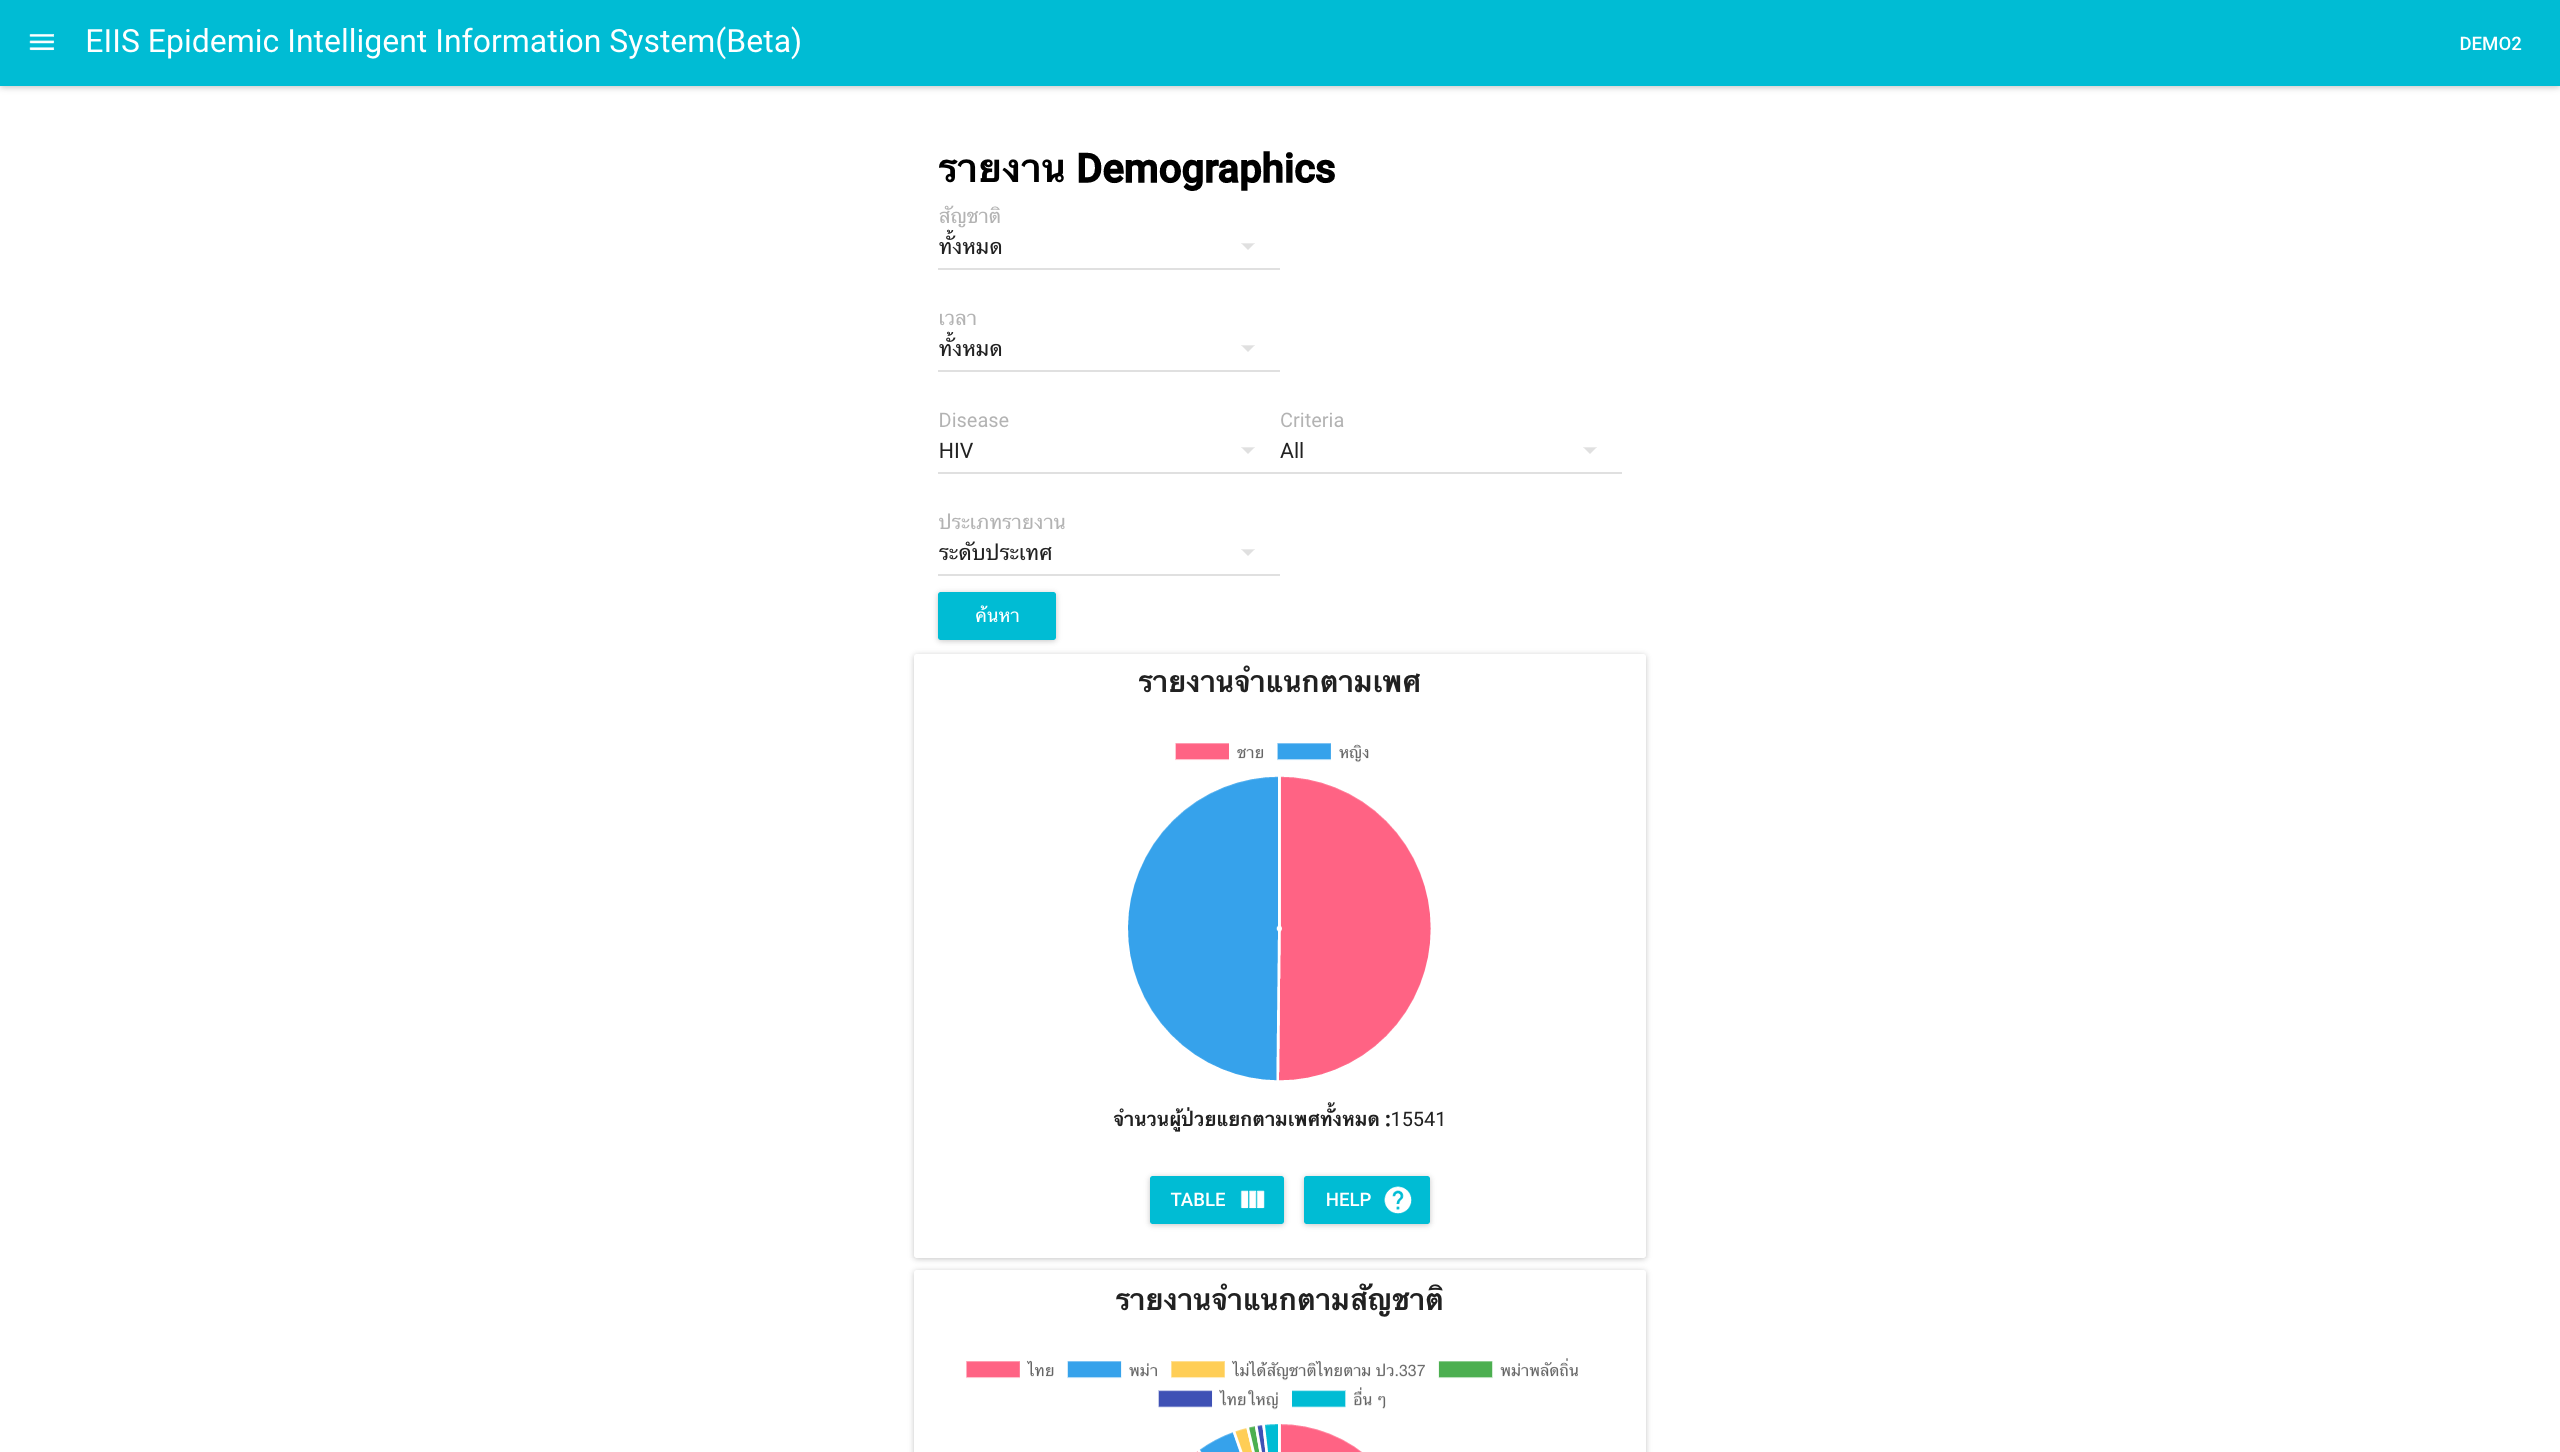
\includegraphics[width=12cm]{images/chapter-05/demographics-report.png}
        		\caption{Demographics Report}
        		\label{demographics-report}
        \end{figure}
	\FloatBarrier
	
	\subsection{Charts} \label{chart}
	   	 
	
    	\subsubsection{Pie Chart separate by Gender}
    	    In this pie chart, it shows the data between male and female. Pink means male and Blue means Women. As it shown in figure \ref{pie-graph-sex}
    	    \vspace{10mm}
        	\FloatBarrier
            	\begin{figure}[h!]
                    \centering
                        % can use width=\linewidth
                		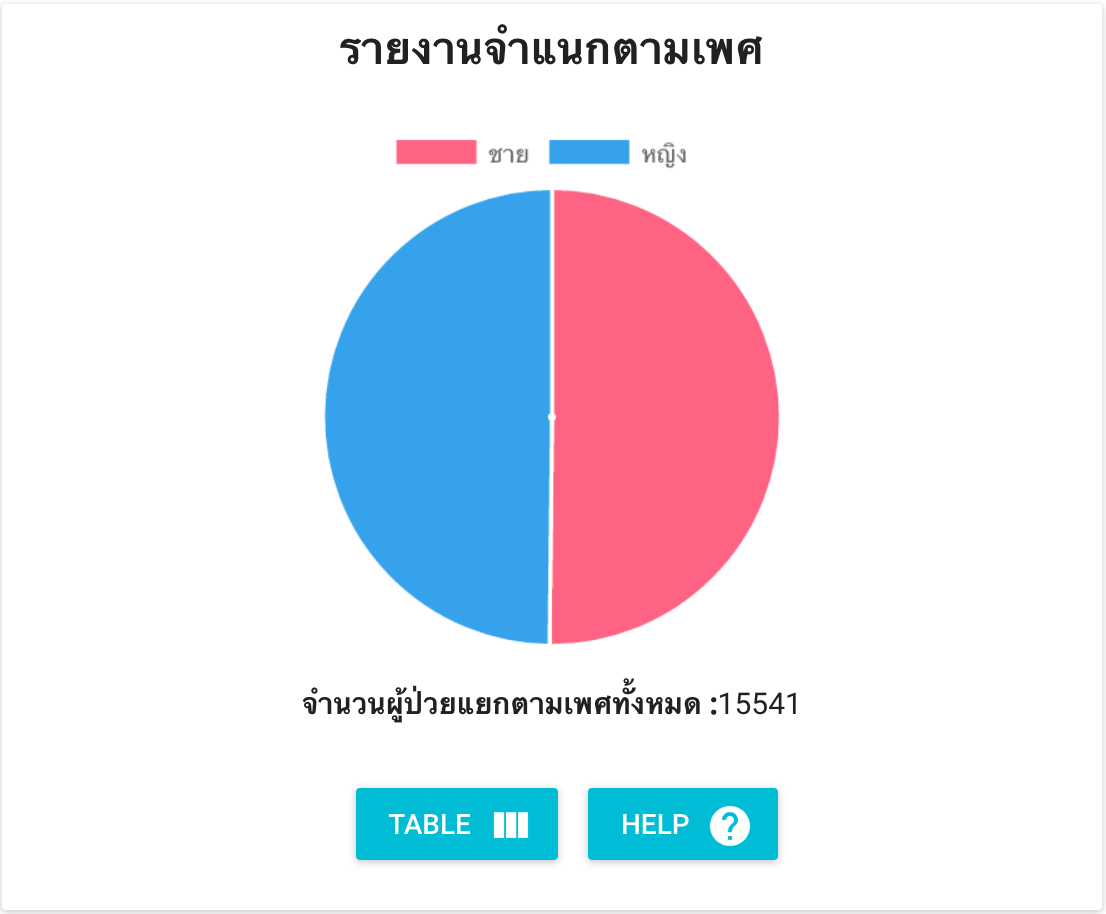
\includegraphics[width=9cm]{images/chapter-05/pie-graph-sex.png}
                		\caption{Gender Pie Chart}
                		\label{pie-graph-sex}
                \end{figure}
        	\FloatBarrier
    	\newpage
        \subsubsection{Pie Chart separate by Nation}
            In this pie chart, it shows data that separated by nation that will be sorted from the top highest. It means that it will show top five that have highest people in that nation and other group will be put in as other. As it shown in figure \ref{pie-graph-nation}
	
        	\FloatBarrier
            	\begin{figure}[h!]
                    \centering
                        % can use width=\linewidth
                		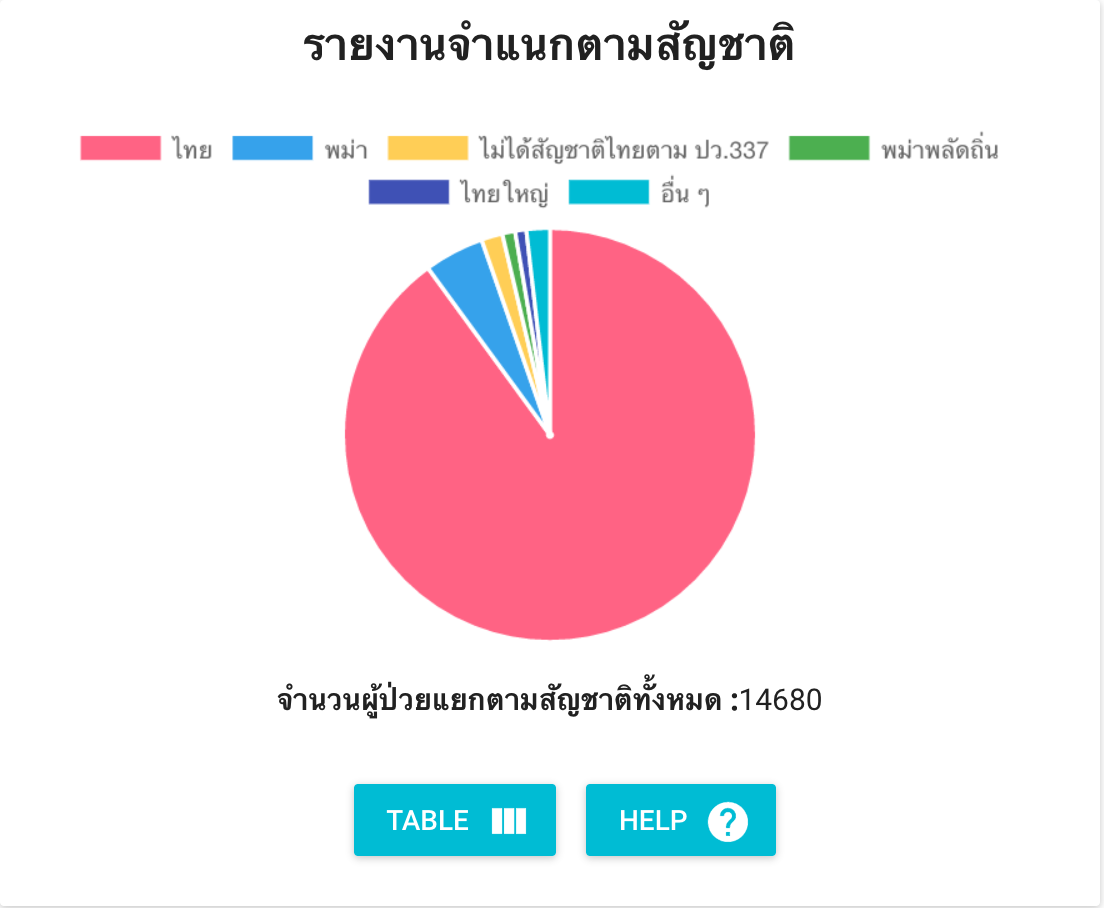
\includegraphics[width=9cm]{images/chapter-05/pie-graph-nation.png}
                		\caption{Nation Pie Chart}
                		\label{pie-graph-nation}
                \end{figure}
        	\FloatBarrier
        \subsubsection{Pie Chart separate by Occupation}
            In this pie chart, it shows data that separated by occupation that will be sorted from the top highest. It means that it will show top four that have highest people on that occupation area and other left will be put as other type. As it shown in figure \ref{pie-graph-occupation}
	
        	\FloatBarrier
            	\begin{figure}[h!]
                    \centering
                        % can use width=\linewidth
                		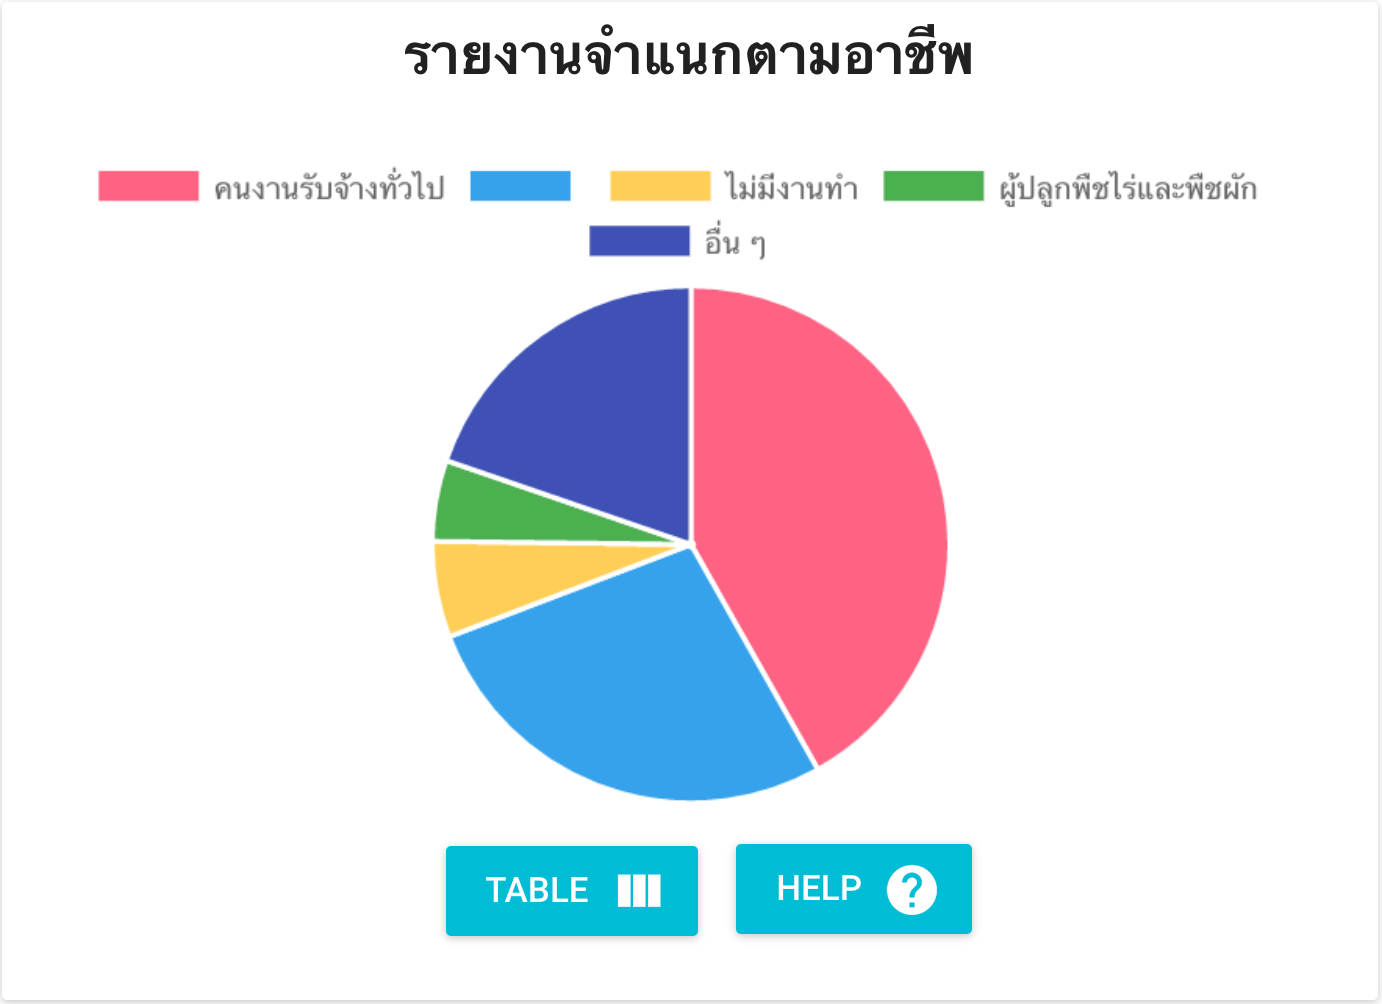
\includegraphics[width=8cm]{images/chapter-05/pie-graph-occupation.png}
                		\caption{Pie Chart separate by Occupation}
                		\label{pie-graph-occupation}
                \end{figure}
        	\FloatBarrier
	
	    \subsubsection{Pie Chart separate by Marital Status}
            In this pie chart, it shows data that separated by status that will be sorted from the top highest. It means that it will show top four that have highest people on that status and other left will be put as other type, as shown in figure \ref{pie-graph-status}
	
        	\FloatBarrier
            	\begin{figure}[h!]
                    \centering
                        % can use width=\linewidth
                		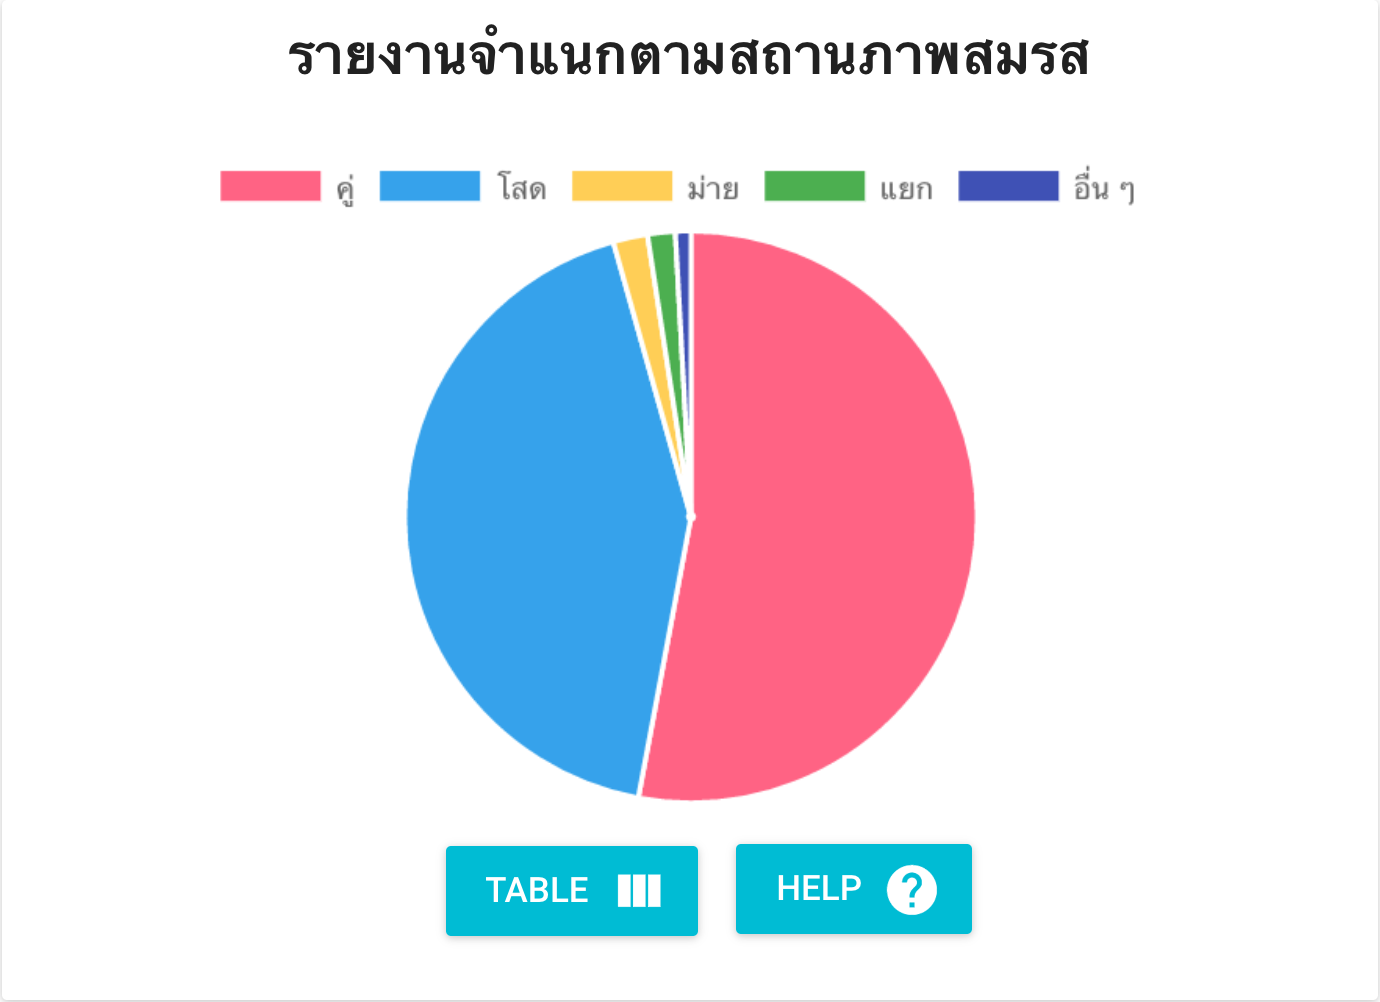
\includegraphics[width=9cm]{images/chapter-05/pie-graph-status.png}
                		\caption{Marital Status Pie Chart}
                		\label{pie-graph-status}
                \end{figure}
        	\FloatBarrier
	
	    \subsubsection{Histogram Separate by Gender}
            In this histogram, it shows histogram that separate data by age and gender. On the horizontal scale will tell you about age. It is ordered from less to high, and in the vertical, it shows the amount number of people. Furthermore, in this graph will compare between male and female as you can see in the graph below. Green means male and orange means female. As it shown in figure \ref{graph-age-sex}
              
    	\FloatBarrier
        	\begin{figure}[h!]
                \centering
                    % can use width=\linewidth
            		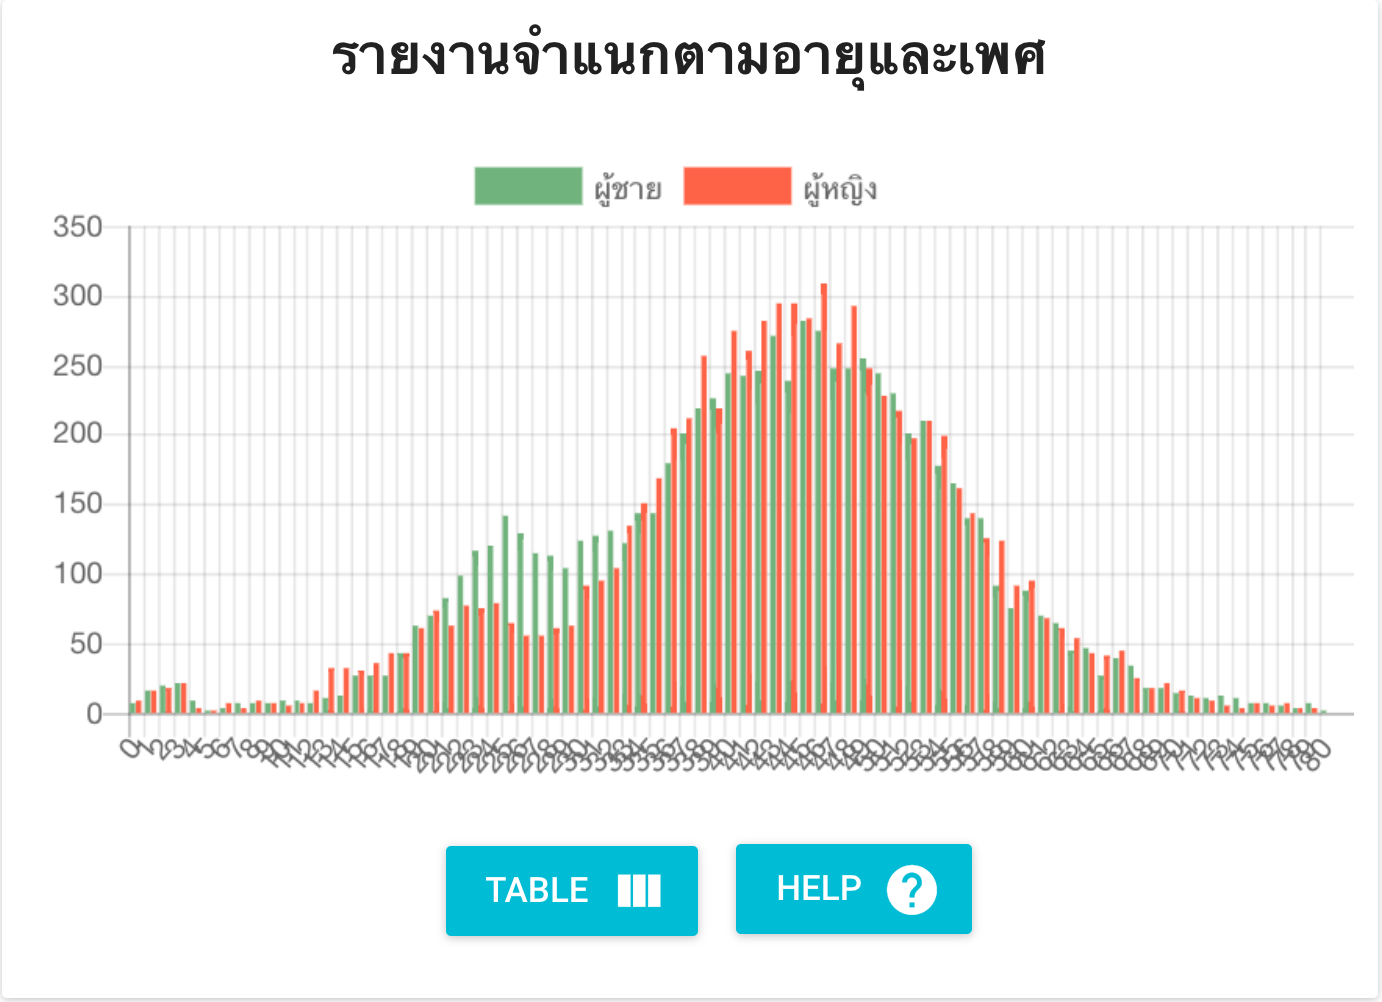
\includegraphics[width=9cm]{images/chapter-05/graph-age-sex.png}
            		\caption{Histogram separate by Gender}
            		\label{graph-age-sex}
            \end{figure}
    	\FloatBarrier
    	
    	\subsubsection{Pie Chart separate by Province}
            In this pie chart, it shows data that separated by province that will be sorted from the top highest. It means that it will show top ten that have highest people on that province area and other left will be put as other type. As it shown in figure \ref{pie-graph-province}
	
    	\FloatBarrier
        	\begin{figure}[h!]
                \centering
                    % can use width=\linewidth
            		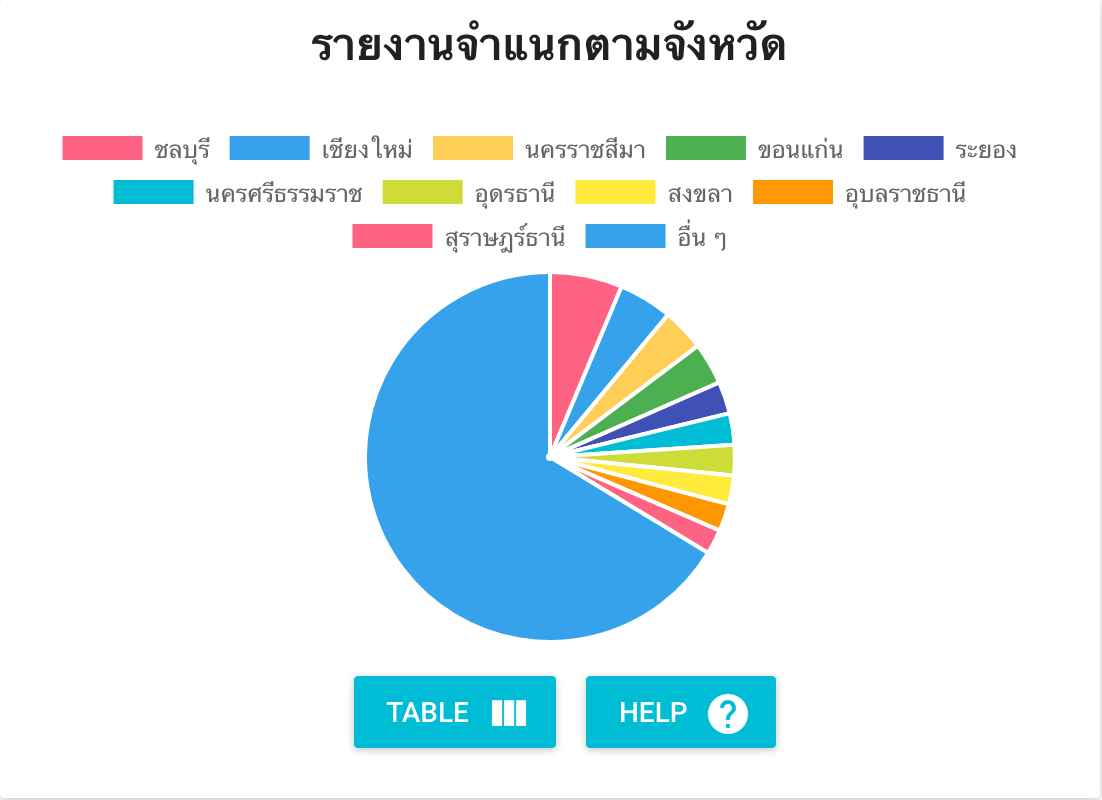
\includegraphics[width=9cm]{images/chapter-05/pie-graph-province.png}
            		\caption{Pie Chart separate by Province}
            		\label{pie-graph-province}
            \end{figure}
    	\FloatBarrier
    	
    	\subsubsection{Pie Chart separate by Hospital}
            In this pie chart, it shows data that separated by hospital that will be sorted from the top highest. It means that it will show top five that have highest people in that hospital and other left will be put as other type. As it shown in figure \ref{pie-graph-hospital}
	
    	\FloatBarrier
        	\begin{figure}[h!]
                \centering
                    % can use width=\linewidth
            		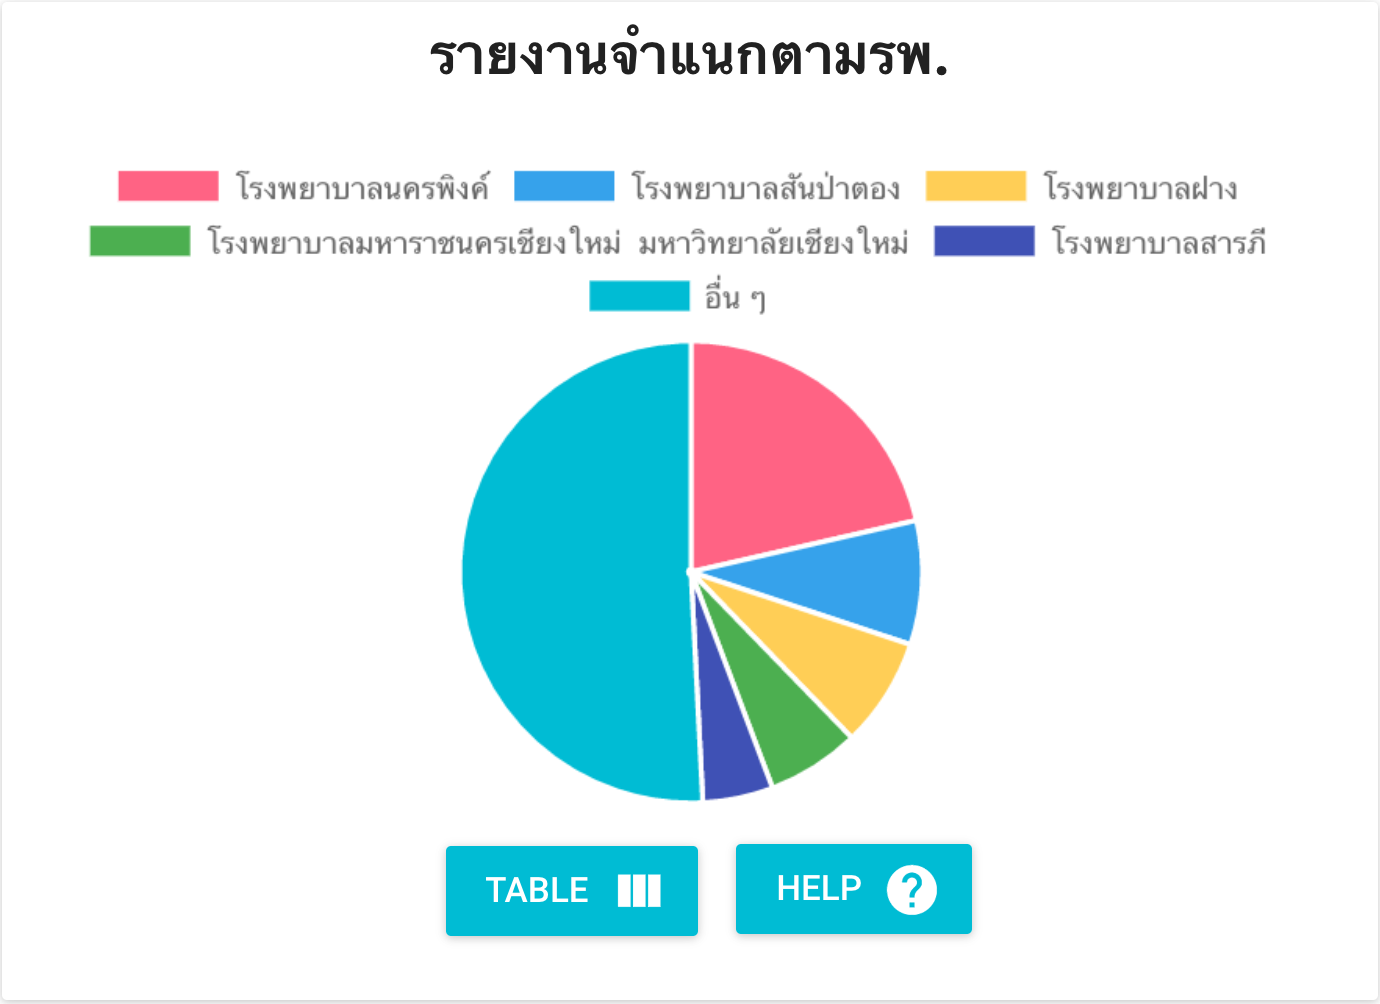
\includegraphics[width=9cm]{images/chapter-05/pie-graph-hospital.png}
            		\caption{Pie Chart separate by Hospital}
            		\label{pie-graph-hospital}
            \end{figure}
    	\FloatBarrier
    	
    	\subsubsection{Pie Chart Between AIDS and Non-AIDS}
    % 	???????????  Aids and non-AIDs
    	   % diagnosis result (Z21,B20X,B21X)by the doctor
            In this pie chart, it shows data that separated between AIDS and Non-AIDS. AIDS means that patient who have the diagnosis result from ICD-10 ( International Statistical Classification of Diseases and Related Health Problems) which are "B20", "B21" and "B22". Non-AIDS means that patient who do not have a lab result. Blue means AIDS and pink means Non-AIDS As the chart shown in figure \ref{pie-graph-seperate-disease}. However, this graph is shown only when user choose HIV in disease drop-down.

    	\FloatBarrier
        	\begin{figure}[h!]
                \centering
                    % can use width=\linewidth
            		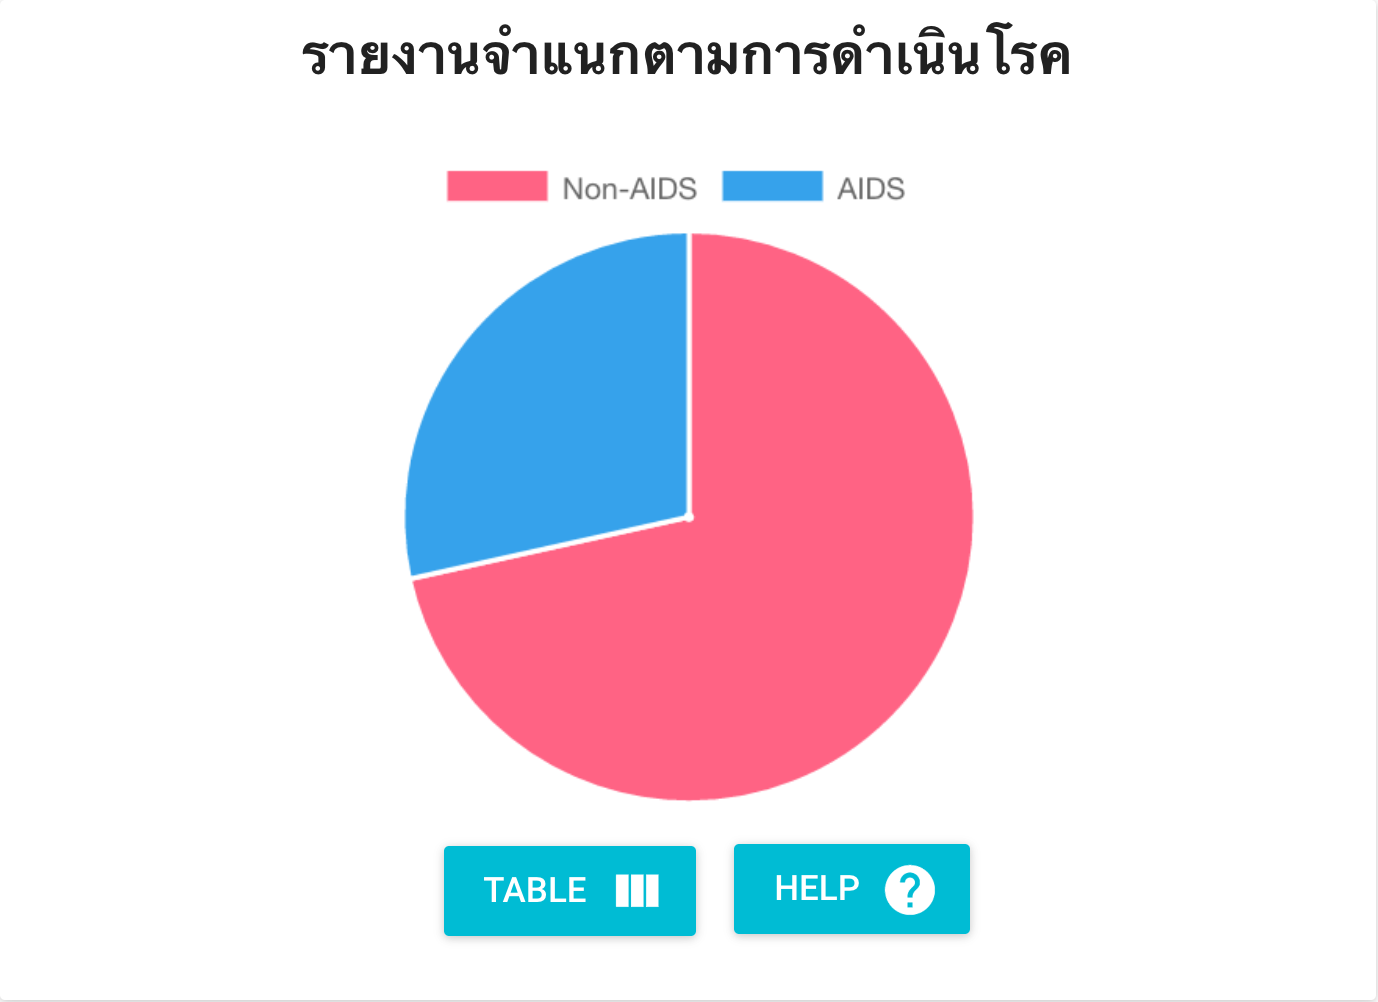
\includegraphics[width=9cm]{images/chapter-05/pie-graph-seperate-disease.png}
            		\caption{Pie Chart Between AIDS and Non-AIDS}
            		\label{pie-graph-seperate-disease}
            \end{figure}
    	\FloatBarrier
	
	
	    \subsubsection{Pie Chart Separate by Medication}
	    
	        This pie chart will show when user select HIV in the disease drop-down. In this pie chart, it shows data that separated by drug. Active drug means patient who have HIV that still get the drug, and inactive drug means patient who have HIV that not get the drug
	        Blue means inactive drug and pink means active drug As the chart shown in figure \ref{pie-graph-receive-medicine}. However, this graph is shown only when user choose HIV in disease drop-down.
	        
           
        	\FloatBarrier
            	\begin{figure}[h!]
                    \centering
                        % can use width=\linewidth
                		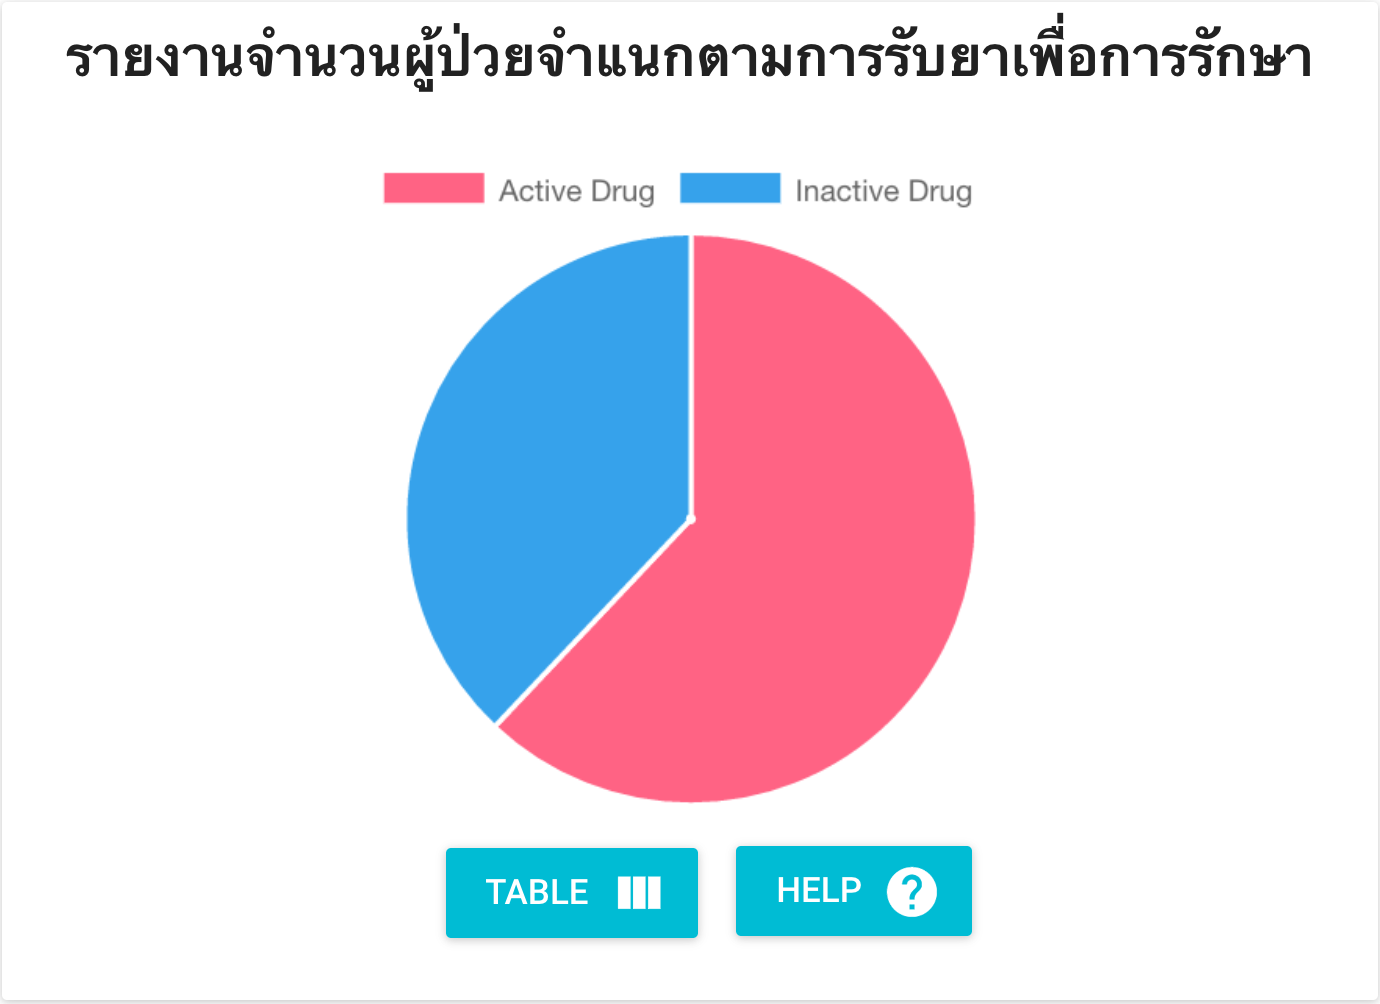
\includegraphics[width=9cm]{images/chapter-05/pie-graph-receive-medicine.png}
                		\caption{Pie Chart Separate by Receiving Drug}
                		\label{pie-graph-receive-medicine}
                \end{figure}
        	\FloatBarrier
	
	
        \subsubsection{Pie Chart Separate by HIV and TB}
        
        	This pie chart is very special because it is the only place that can show pie chart that separate by HIV and TB. The reason that it is very special is because the data(43 folder), that we received, can analysis and show the pie chart that can count people who have HIV and TB at the same time. This pie chart shows data that separated by TB and Non-TB. TB here means patient who have HIV and also have TB as represented in blue and Non-TB means patient who have HIV but do not have TB as represented in pink. As the pie chart is shown in figure \ref{pie-graph-hiv-tb}. However, this graph is shown only when user choose HIV in disease drop-down.
    	
    	\FloatBarrier
        	\begin{figure}[h!]
                \centering
                    % can use width=\linewidth
            		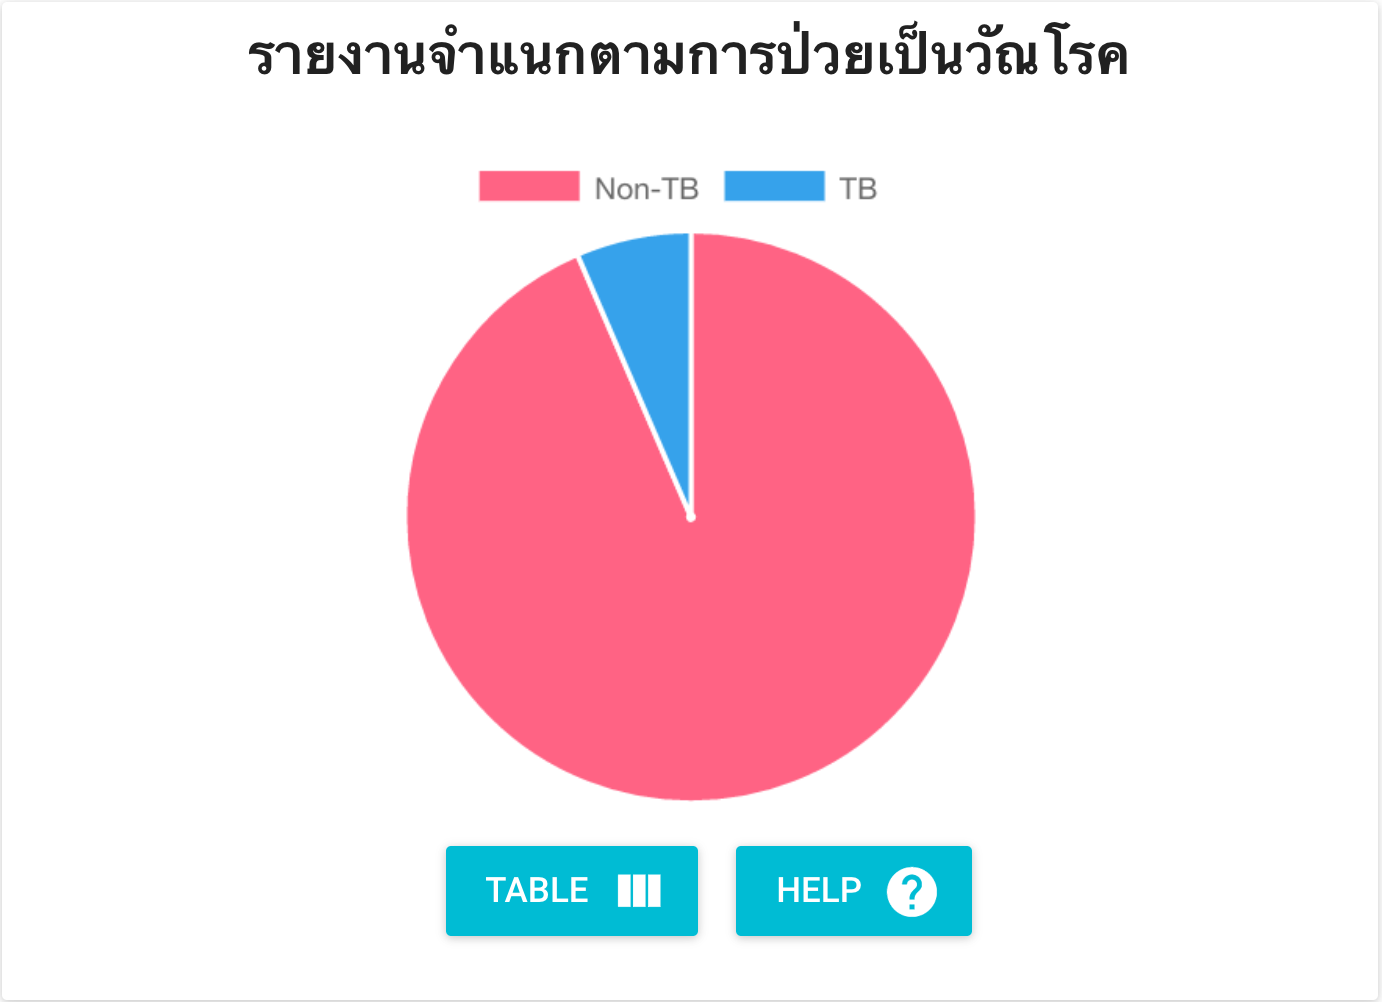
\includegraphics[width=9cm]{images/chapter-05/pie-graph-hiv-tb.png}
            		\caption{HIV TB Pie Chart}
            		\label{pie-graph-hiv-tb}
            \end{figure}
    	\FloatBarrier
    	
    	\subsubsection{HIV Follow Up Chart}
    	
    	In this bar chart, it will show HIV follow up, the purpose of this graph is to follow the patient who have HIV. There are five main bar in this chart which are patient who have HIV, on ARV, last visit(in a year), viral load in a year, and viral suppressed. In the horizontal scale, there will be the topics and the vertical scale will be the amount of people. the first bar means people who have HIV, so it will count the people who have HIV. The second bar (on ARV) means people who have to get Antiretroviral drugs. The third bar means patient who last visit to hospital in the a year. the fourth bar(viral load in a year) means patient who go to check viral load in a year which patient can go check at hospital. The last bar(viral suppressed) means patient who go to check viral load in a year and the value is low.

	
    	\FloatBarrier
        	\begin{figure}[h!]
                \centering
                    % can use width=\linewidth
            		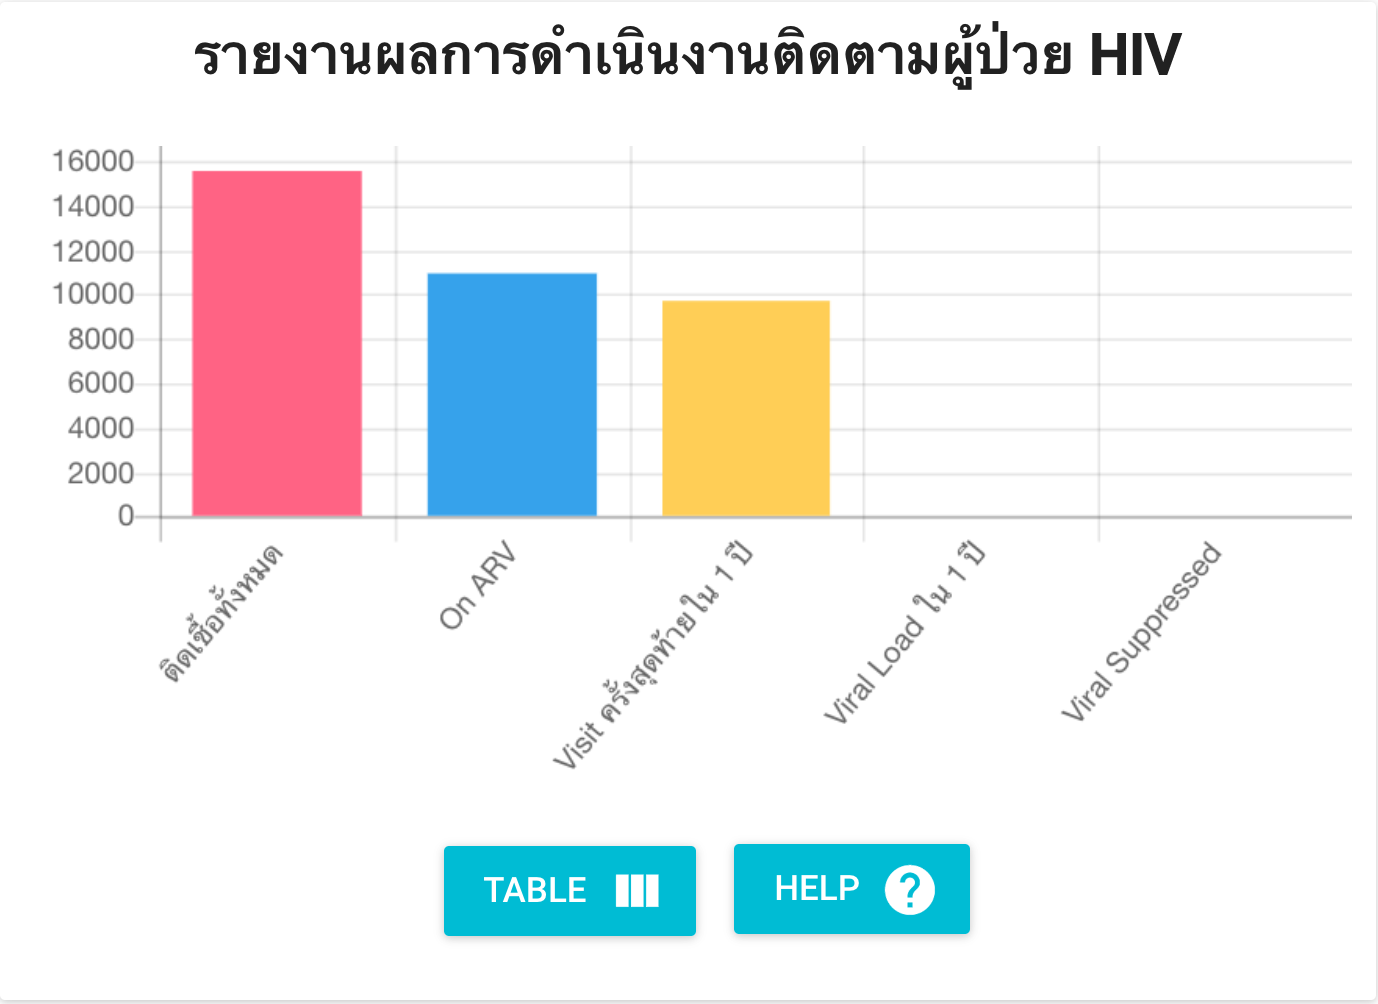
\includegraphics[width=9cm]{images/chapter-05/pie-graph-follow-hiv.png}
            		\caption{HIV Follow Up Chart}
            		\label{pie-graph-follow-hiv}
            \end{figure}
    	\FloatBarrier
	
% 	\subsection{Individual Report}
	
	\subsection{Log-Out}
	
	
	To log-out, user need to select log-out in tab bar menu that shown in figure \ref{log-out}.  After that the front-end will use POST method as /api/v1/auth/logout in order to log-out. After that it will bring you to the log-in page as shown in figure \ref{log-in}.
	
	\vspace{10mm}
    \FloatBarrier
    	\begin{figure}[h!]
            \centering
                % can use width=\linewidth
        		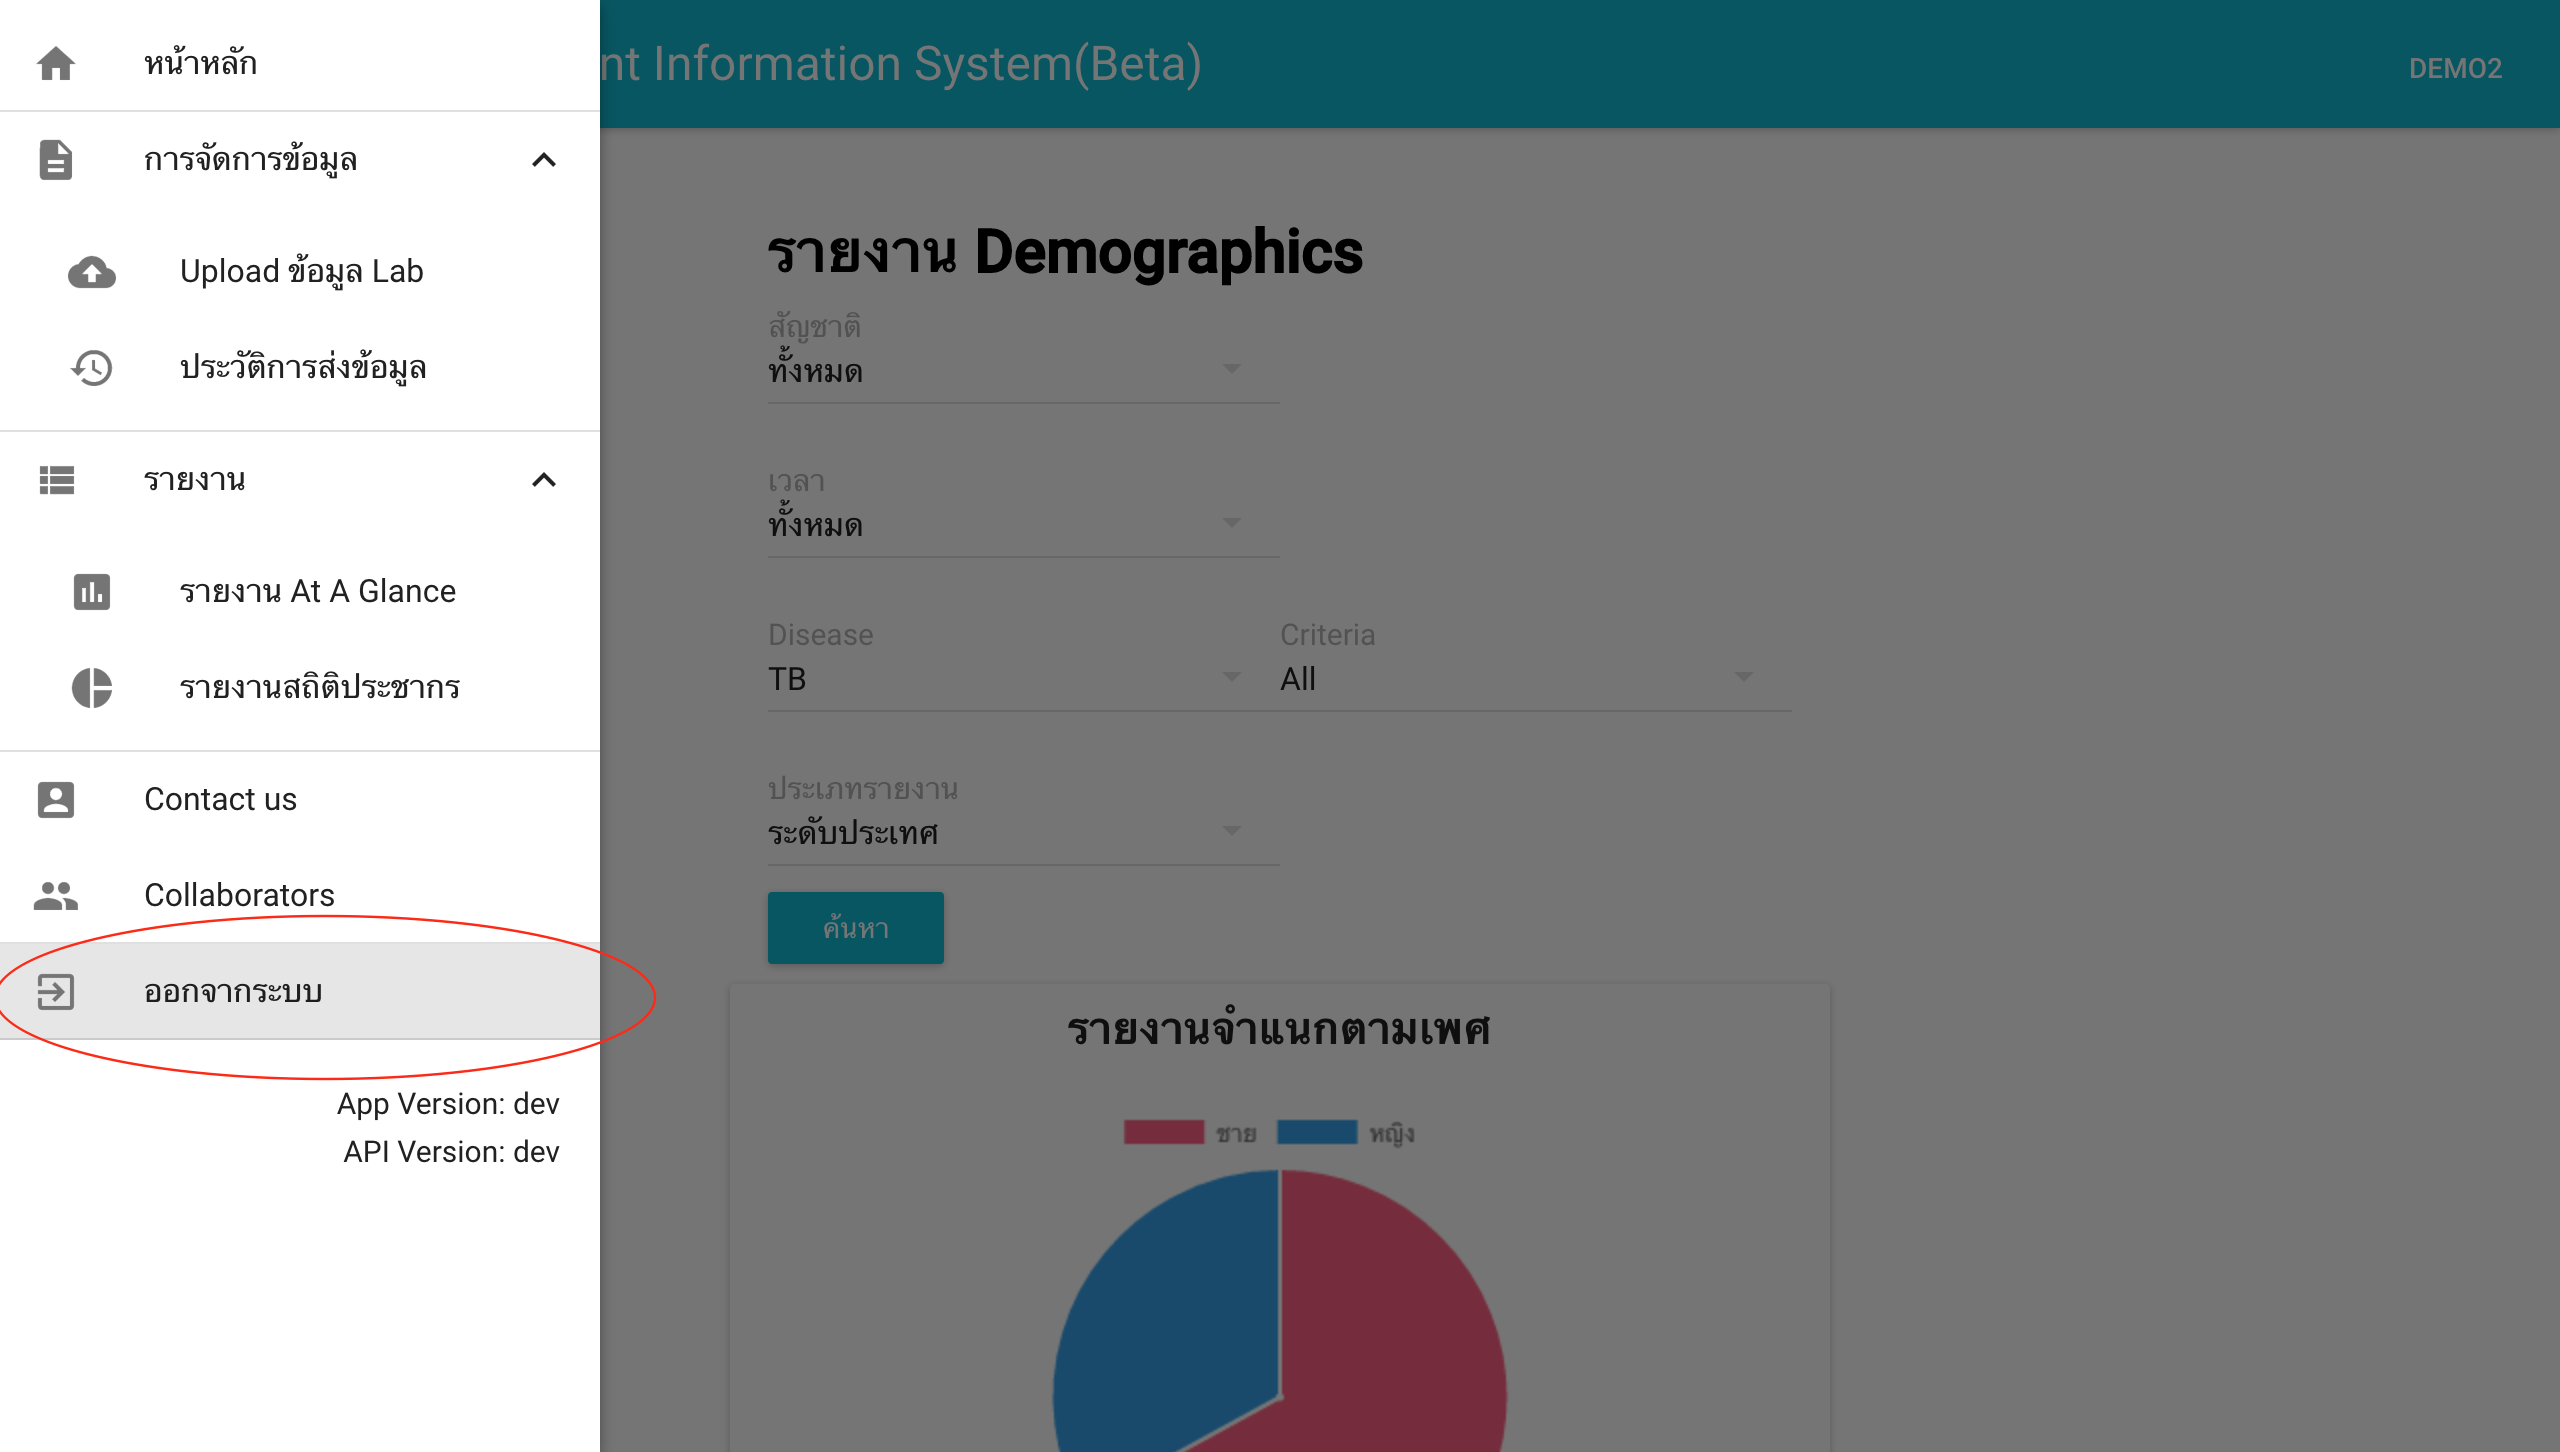
\includegraphics[width=10cm]{images/chapter-05/log-out.png}
        		\caption{Log-Out}
        		\label{log-out}
        \end{figure}
	\FloatBarrier